%%
%% Copyright 2007, 2008, 2009 Elsevier Ltd
%%
%% This file is part of the 'Elsarticle Bundle'.
%% ---------------------------------------------
%%
%% It may be distributed under the conditions of the LaTeX Project Public
%% License, either version 1.2 of this license or (at your option) any
%% later version.  The latest version of this license is in
%%    http://www.latex-project.org/lppl.txt
%% and version 1.2 or later is part of all distributions of LaTeX
%% version 1999/12/01 or later.
%%
%% The list of all files belonging to the 'Elsarticle Bundle' is
%% given in the file `manifest.txt'.
%%

%% Template article for Elsevier's document class `elsarticle'
%% with numbered style bibliographic references
%% SP 2008/03/01

%%\documentclass[doublespacing]{elsarticle}
\documentclass[preprint, 10pt]{elsarticle}

%% Use the option review to obtain double line spacing
%% \documentclass[authoryear,preprint,review,12pt]{elsarticle}

%% Use the options 1p,twocolumn; 3p; 3p,twocolumn; 5p; or 5p,twocolumn
%% for a journal layout:
%% \documentclass[final,1p,times]{elsarticle}
%% \documentclass[final,1p,times,twocolumn]{elsarticle}
%\documentclass[final,3p, times]{elsarticle}
%% \documentclass[final,3p,times,twocolumn]{elsarticle}
%% \documentclass[final,5p,times]{elsarticle}
%% \documentclass[final,5p,times,twocolumn]{elsarticle}

%% For including figures, graphicx.sty has been loaded in
%% elsarticle.cls. If you prefer to use the old commands
%% please give \usepackage{epsfig}

%% The amssymb package provides various useful mathematical symbols
\usepackage{amsmath}
\usepackage{amssymb}
\usepackage{mathtools}
%\usepackage[linesnumbered, ruled, vlined]{algorithm2e}
\usepackage{algorithm}% http://ctan.org/pkg/algorithms
\usepackage{algorithmicx}
\usepackage{algpseudocode}% http://ctan.org/pkg/algorithmicx
\renewcommand{\algorithmicrequire}{\textbf{Input:}}
\renewcommand{\algorithmicensure}{\textbf{Output:}}
\usepackage{enumerate}
\usepackage{multirow}
\usepackage{graphicx}
\usepackage{subfigure}
\usepackage{epstopdf}

\usepackage{booktabs}
\usepackage[dvipsnames]{xcolor}
\usepackage{tcolorbox}
\usepackage{soul}
%\tcbset{enhanced jigsaw, sharp corners,box align=center,boxrule=0pt}

\usepackage{lineno}

\usepackage{indentfirst}
%Bibliography
\usepackage{natbib}
\usepackage{hypernat}

\usepackage{lipsum} % Package to generate dummy text throughout this template

%\usepackage[sc]{mathpazo} % Use the Palatino font
\usepackage[T1]{fontenc} % Use 8-bit encoding that has 256 glyphs
%\linespread{2} % Line spacing - Palatino needs more space between lines
\usepackage{microtype} % Slightly tweak font spacing for aesthetics

\usepackage[hmarginratio=1:1,top=32mm,columnsep=20pt]{geometry} % Document margins
\usepackage{multicol} % Used for the two-column layout of the document
\usepackage[hang, small,labelfont=bf,up,textfont=it,up]{caption} % Custom captions under/above floats in tables or figures
\usepackage{booktabs} % Horizontal rules in tables
\usepackage{float} % Required for tables and figures in the multi-column environment - they need to be placed in specific locations with the [H] (e.g. \begin{table}[H])
\usepackage{hyperref} % For hyperlinks in the PDF

\usepackage{lettrine} % The lettrine is the first enlarged letter at the beginning of the text

\usepackage{amsthm,amsmath,amssymb}
\usepackage{mathrsfs}
\usepackage[section]{placeins}
%\usepackage{refcheck} % check the reference of equations, figures, tables and citations


\journal{Journal of Computational Physics}

\begin{document}
%	\linenumbers
	
\begin{frontmatter}

%% Title, authors and addresses

%% use the tnoteref command within \title for footnotes;
%% use the tnotetext command for theassociated footnote;
%% use the fnref command within \author or \address for footnotes;
%% use the fntext command for theassociated footnote;
%% use the corref command within \author for corresponding author footnotes;
%% use the cortext command for theassociated footnote;
%% use the ead command for the email address,
%% and the form \ead[url] for the home page:
%% \title{Title\tnoteref{label1}}
%% \tnotetext[label1]{}
%% \author{Name\corref{cor1}\fnref{label2}}
%% \ead{email address}
%% \ead[url]{home page}
%% \fntext[label2]{}
%% \cortext[cor1]{}
%% \address{Address\fnref{label3}}
%% \fntext[label3]{}

\title{Physics-informed machine learning for reduced-order modelling }

%% use optional labels to link authors explicitly to addresses:
%% \author[label1,label2]{}
%% \address[label1]{}
%% \address[label2]{}

\author[XJTU]{Wenqian Chen}
\ead{wenqianchen2016@gmail.com}
\author[EPFL]{Qian Wang\corref{cor1}}
\cortext[cor1]{Corresponding author.}
\ead{qian.wang@epfl.ch}
\author[EPFL]{Jan S. Hesthaven}
\ead{Jan.Hesthaven@epfl.ch}
\author[XJTU]{Chuhua Zhang}
\ead{chzhang@mail.xjtu.edu.cn}
\address[XJTU]{Department of Fluid Machinery and Engineering, School of Energy and Power Engineering, Xi'an Jiaotong University, Xi'an, Shaanxi, People's Republic of China}
\address[EPFL]{Chair of Computational Mathematics and Simulation Science, \'Ecole polytechnique f\'ed\'erale de Lausanne, 1015 Lausanne, Switzerland}

\begin{abstract}
%% Text of abstract
  \hspace{8pt} A physics-informed machine learning framework is developed for the reduced-order modeling of parametirzed steady-state partial differential equations (PDEs). In the offline stage, a reduced-order model is constructed by projecting the high-fidelity numerical model onto a reduced space, spanned by a set of reduced basis that represents the main dynamics of the full-order model. A physics-informed neural network (PINN) and a physics-reinforced neural network (PRNN) are developed to approximate the mapping from the parameters to the projection coefficients. The former is trained by minimizing the residual of the reduced-order model, while the latter is trained by minimizing the residual in combination with the matching error between  the projection coefficients and network outputs. In the online stage, given a new parameter location, the projection coefficients are predicted by the neural networks. Numerical results demonstrate that the PINN and PRNN can provide more accurate solutions to nonlinear problems with fewer high-fidelity solutions, compared with a non-intrusive reduced-order method. Besides, the PRNN are validated more accurate and robust than the PINN for complex nonlinear problems.

\end{abstract}

\begin{keyword}
%% keywords here, in the form: keyword \sep keyword
   physics-informed machine learning \sep Neural network  \sep reduced-order modeling \sep nonlinear PDE

%% PACS codes here, in the form: \PACS code \sep code

%% MSC codes here, in the form: \MSC code \sep code
%% or \MSC[2008] code \sep code (2000 is the default)

\end{keyword}

\end{frontmatter}

%\linenumbers

%% main text
\section{Introduction}
In recent years, although high-fidelity numerical method has witnessed substantial developments for modeling complex phenomena, it is still challenging for many applications, such as design, optimization, control and uncertainty quantification problems. Such applications are governed by parameterized partial differential equations(PDEs) \cite{hesthaven2016certified, quarteroni2015reduced}, where parameters characterize underlying geometry, boundary conditions, source terms and physical properties, etc. High-fidelity numerical method are prohibitively expensive to such applications in multi-entry and real-time contexts, due to the required lots of degrees of freedom(DOFs).
%Although increasing computational power and parallel techniques are nowadays available to largely reduce the consumed wall time, the total cost with respect to both consumed CPU time and money remains prohibitively expensive.
The need to largely reduce computational cost gives birth to reduced-order modeling methods \cite{lucia2004reduced}, aiming at replacing the full-order system with a cheap reduced-order system with an affordable loss of accuracy.


Reduced basis (RB) method is one of the well-known and widely-used reduced-order modeling methods, and always follows the offline-online paradigm \cite{maday2006reduced}. The offline stage comprises preparing high-fidelity solutions(snapshots), extracting the reduced basis and building a cheap evaluation model. The reduced space, spanned by the reduced basis  extracted from the snapshots, is expected to represent the main dynamics of the full-order model. There exist many methods to extract the reduced basis, such as the Proper Orthogonal Decomposition (POD) \cite{hesthaven2016certified,liang2002proper,quarteroni2015reduced}, the  Proper Generalized Decomposition \cite{chinesta2011short}, the Piecewise Tangential Interpolation \cite{gallivan2002model}, the Matrix Interpolation \cite{panzer2010parametric}, greedy algorithms\cite{billaud2017dynamical, lappano2016greedy, hesthaven2014efficient}. Among them, the POD perhaps is the most widely-known and widely-used one, where the reduced basis is generated by a singular value decomposition (SVD) algorithm for some given snapshots with respect to a chosen set of parameters. After the reduced basis has been properly set up, an approximation to high-fidelity solution is recovered from projection coefficients of the reduced space. Then a suitable model will be built offline, aiming to provide online evaluation for a new given parameter.
For building such a model, both 'white-box' and 'black-box' strategies are applied in the literature.

Galerkin method \cite{rowley2004model, wang2020recurrent, deane1991low} is one of widely-used white-box strategies. In the offline stage,
a reduced-order model determining projection coefficients is derived from Galerkin projection of the full-order model. In the online stage, the reduced-order model is solved by a suitable numerical solver for each parameter.
As projection coefficients are directly solved by a deterministic method, the achieved approximation accuracy is always very good. What's more, no more extra snapshots is required besides the snapshots for building RB.
However, the online solving of the reduced-order model is not trivial, which remains an open problem with respect to its accuracy, stability and convergence \cite{huang2018challenges, iollo2000stability, rowley2004model}. Besides, the online solving of the reduced-order model is still time consuming especially for complex nonlinear problems, even if it is much cheaper than the solving of full-order model.

%Many works have been devoted to improve the stability and accuracy, such as the structure-preservation, supremizer enrichment,basis adaption, L1-norm minimization, and least-squares. Petrov-Galerkin (LSPG) technique.

The black-box strategy is also termed as an non-intrusive procedure, in which the building and also the solving of reduced-order model is avoided. Usually, the high-fidelity simulations producing snapshots are treated as a black box and recovered with a machine learning model.
During the offline stage, a map between the parameter values and the projection coefficients is built by a data-driven way. During the online stage, the projection coefficients for new parameter values can be recovered as outputs of the machine learning model.  For example, non-intrusive approaches using radial basis function (RBF) \cite{chen2018greedy, walton2013reduced, xiao2015non}, artificial neural network(ANN) \cite{hesthaven2018non} and Gaussion process regression(GPR) \cite{guo2019data} have been applied successively for parameterized partial differential equations, even for flow problems of strong nonlinearity. These approaches benefit from their high established effectiveness and efficient online evaluation. However, the drawback, common for data-driven method, is their requirement for an excessive number of observed data to guarantee accuracy. That is to say, many high-fidelity solutions have to be precomputed,  sometimes leading to an unacceptable cost even if it is performed in the offline stage \cite{hesthaven2018non}.


The white-box Galerkin method targets the full-order model, while the black-box machine learning models target high-fidelity solutions. These two strategies approximate the parameterized PDEs in different directions.
In this work,  we try to develop a physics-informed machine learning framework using a grey-box strategy to take the advantages of the above two strategies.
Inspired by the well-know physics-informed neural network (PINN) \cite{raissi2019physics, raissi2020hidden, mao2020physics}, we can directly solve the reduced-order model by  optimizing a neural network.
Thus, we keep on the intrusive approach and utilize the reduced-order information to build a neural network.
For the PINN approach, there is no need for labeled data, thus no need for extra snapshots, and what we need to do is to train a network to satisfy the reduced-order model in some sense.
Besides this approach,  the projection coefficients of snapshots can also be added into the training of network, although they are not the solutions of the reduced-order model. we term this approach as the physics-reinforced neural network (PRNN).
For both PINN and PRNN approaches, they enjoy a higher accuracy and independence of extra snapshots inherited from Galerkin method, and also the effectiveness inherited from machine learning models.
To test this assertion, the PINN and PRNN are applied to one-dimensional Burges' equation, two-dimensional lid-driven flow and natural convection in enclosure. A detailed comparison with the white-box POD-G method and the black-box POD-NN method proposed by Jan et al.\cite{hesthaven2018non} is analysed for the three test cases.

The remainder of this paper is organized as follows. Section 2 presents the framework from parameterized PDEs to the reduced-order model. Section 3 briefly introduce the POD-NN method (referred to PDNN in this work) and presents the derivation of PINN and PRNN method based on the reduced-order information. Section 4 details some numerical setups for these methods, and offers some numerical results to show the superiority of the proposed PINN and PRNN methods, In Section 5, some conclusions are given.

\section{Projection-based reduced basis method}\label{sec:POD-G}
Consider a nonlinear dynamic system governed by the following parameterized partial differential equations(PDEs):
\begin{equation}
\begin{aligned}
\mathcal{N}\left(\phi\left(\mathbf{x}\right); \pmb{\mu}\right)=0&,  \qquad \mathbf{x} \in \Omega\left(\pmb{\mu}\right),  \\
\mathcal{B}\left(\phi\left(\mathbf{x}\right); \pmb{\mu}\right)=0&,  \qquad \mathbf{x} \in \partial \Omega\left(\pmb{\mu}\right),
\end{aligned}
\label{eq_GoverningEqs}
\end{equation}
where $\mathcal{N}$ is a general nonlinear differential operator, $\phi\left(\mathbf{x}\right)$ are field variables to be solved on Cartesian coordinates $\mathbf{x}$. $\mathcal{B}$ are operators defining boundary conditions for the boundary $\partial \Omega$ of the physical  domain $\Omega$. $\pmb{\mu} \in \mathcal{P}$ are specific parameters characterizing the nonlinear dynamic system as well as the physical domain $\Omega$, where $\mathcal{P}$ is the parameter space.

As is always the case for reduced-order methods, a dynamic system is approximated by finding the its projection in a space spanned by a few well-chosen basis vectors. These basis are generated from a suitable linear combination of some precomputed high-fidelity approximations, termed as snapshots. To ensure the compatibility among snapshots, the variable physical domain has to be addressed. To this end, the variable physical domain will be mapped into a fixed computational domain with the same collation of degrees of freedom. This can be implemented by an invertible problem-dependent mapping $\mathcal{X} : \mathbf{x} \in \Omega\left(\pmb{\mu}\right) \to \pmb{ \xi} \in \widetilde \Omega$, which reads
\begin{equation}
\pmb{ \xi} = \mathcal{X} \left( \mathbf{x}; \pmb{\mu} \right),
\label{eq_Transform}
\end{equation}
and thus the governing equations (\ref{eq_GoverningEqs}) are recast as follows:
\begin{equation}
\begin{aligned}
\mathcal{N}\left(\phi\left( \mathcal{X}^{-1} \left( \pmb{ \xi}; \pmb{\mu} \right) \right); \pmb{\mu}\right)
&:=\widetilde {\mathcal{N}} \left(\phi\left( \pmb{ \xi} \right); \pmb{\mu}\right)
=0,  \qquad \pmb{ \xi} \in \widetilde \Omega,
\\
\mathcal{B}\left(\phi\left(\mathcal{X}^{-1} \left( \pmb{ \xi}; \pmb{\mu} \right)\right); \pmb{\mu}\right)
&:=\widetilde {\mathcal{B}} \left(\phi\left( \pmb{ \xi} \right); \pmb{\mu}\right)
=0,  \qquad \pmb{ \xi} \in \partial \widetilde \Omega,
\end{aligned}
\label{eq_GoverningEqsForXi}
\end{equation}
where $\widetilde \Omega$ is the computational domain, $\widetilde {\mathcal{B}}$ and $\widetilde {\mathcal{N}}$ are the derived operators in computational space resulting from the transformation Eq. (\ref{eq_Transform}).

\subsection{Full-order model}
To simulate the nonlinear dynamic system in Eqs. (\ref{eq_GoverningEqsForXi}), the including spatial derivatives are always first discretized by a suitable high-fidelity (HF) method (such as the Chebyshev pseudospectral method \cite{chen2018multidomain, chen2020parallel}, spectral difference method \cite{chen2020collocated}, etc.). To achieve a satisfactory numerical accuracy, a fine mesh is employed with a large number of degrees of freedom (DOFs), generally including $N$ interior DOFs and $N_B$ boundary DOFs. Finally, the resulting discretized equations for  Eqs. (\ref{eq_GoverningEqsForXi}) are solved with a suitable explicit/implicit solver.

Here we denote the discrete solutions of Eq ( \ref{eq_GoverningEqsForXi}) in vector form $\pmb{\phi} _h \in \mathbf{R}^{N  }$ and $\pmb{\phi} _h^{B} \in \mathbf{R}^{N_B}$ for parameter $\pmb{\mu}  \in \mathcal{P}$.
Given a suitable HF method, we have the governing Eq. (\ref{eq_GoverningEqsForXi}) in discrete form
\begin{align}
\mathbf{L}_{\widetilde {\mathcal{N}}}\pmb{\phi}_h +g_{\widetilde {\mathcal{N}}}(\pmb{\phi}_h, \pmb{\phi}_h^{B})
+\mathbf{C}_{\widetilde {\mathcal{N}}}
= 0,
\label{eq_DiscreteEqs}
\\
\mathbf{L}_{\widetilde {\mathcal{B}}} \pmb{\phi}_h + \mathbf{L}_{\widetilde {\mathcal{B}}}^{B} \pmb{\phi}_h^{B}
+\mathbf{C}_{\widetilde {\mathcal{B}}}
= 0,
\label{eq_DiscreteBoundary}
\end{align}
where $\mathbf{L}_{\widetilde {\mathcal{N}}} \in \mathbf{R}^{N \times N}$, $\mathbf{L}_{\widetilde {\mathcal{B}}} \in \mathbf{R}^{N_B \times N}$ and $\mathbf{L}_{\widetilde {\mathcal{B}}}^{B} \in \mathbf{R}^{N_B \times N_B}$ represent matrixes derived from linear parts of operators $\widetilde {\mathcal{N}}$ and $\widetilde {\mathcal{B}}$.
$\mathbf{C}_{\widetilde {\mathcal{N}}} \in \mathbf{R}^{N}$ and $\mathbf{C}_{\widetilde {\mathcal{B}}} \in \mathbf{R}^{N_B}$ are constant vectors independent of $\pmb{\phi} _h$ and $\pmb{\phi} _h^B$.
$g_{\widetilde {\mathcal{N}}}: \mathbf{R}^N \times \mathbf{R}^{N_B} \mapsto \mathbf{R}^N$ is a nonlinear function derived from the nonlinear part of operator $\widetilde {\mathcal{N}}$.

For the treatment of boundary conditions, it can be classified into two categories, namely weakly enforced and strongly enforced boundary conditions.
As for weakly enforced boundary conditions, no DOFs is required to deploy on the boundaries, i.e. $N_B=0$, implying a vanishing of $\pmb{\phi} _h^{B}$ and also Eq. (\ref{eq_DiscreteBoundary}). As for strongly enforced boundary conditions, a suitable collocation of DOFs on boundaries is necessary. Note that the commonly used boundary conditions always linear ones, such as Dirictlet, Neumann and Robin conditions, and thus $\mathcal{B}$ are always linear operators. Without loss of generality, we restrict ourselves that the mapping in Eq. (\ref{eq_Transform}) will retain the linearity of boundary condition operator $\widetilde {\mathcal{B}}$ in computational space. Therefore, discretization of the boundary conditions result in a linear system of equations, i.e., Eq. (\ref{eq_DiscreteBoundary}).

In what remains, the Chebyshev pseudospectral method, characterized by its outstanding accuracy, is chosen for discretizing Eqs. (\ref{eq_GoverningEqsForXi}),  which will be detailed in the following subsection.

\subsubsection{Chebyshev pseudospectral method}
In the Chebyshev pseudospectral method, the $d$-dimensional variable physical domain of  will be mapped into a unit regular computational domain $\widetilde \Omega =[-1,1]^d$,  each dimension discretized by  $N_p+1$ Chebyshev-Gauss-Lobatto points,
\begin{equation}
\xi_i=\cos \left( \frac{\pi i}{N_p} \right), \quad 0 \le i \le {N_p}.
\label{eq_CollocationPoints}
\end{equation}
Spatial derivatives in operators $\widetilde {\mathcal{N}}$ and $\widetilde {\mathcal{B}}$ are approximated with a matrix-vector multiplication in each dimension. In each dimension, the derivatives are approximated as follows:
\begin{equation}
\left. { \frac{\partial^s    \phi}{{\partial \xi^s}  }} \right|_{\xi _i }
 = \mathbf{D}^s \pmb{\phi},
\end{equation}
where $\pmb{\phi}=\{\phi _i\}_{i=0}^{N_p}$, $s$ is the order of derivative and $\mathbf{D}^s$ is the $s$th-order difference matrix of size ${(N_p+1)\times (N_p+1)}$ with entries defined by
\begin{equation}
D^0_{i,j} = \delta_{ij}, \qquad 0 \le i,j \le {N_p},
\label{eq_D0}
\end{equation}
\begin{equation}
\left\{ \begin{aligned}
&D_{i,j}^1 = \frac{{{B_i}}}{{{B_j}}}\frac{{{{( - 1)}^{i + n}}}}{{2\sin \left( {\frac{{(i + j)\pi }}{{2{N_x}}}} \right)\sin \left( {\frac{{(j - i)\pi }}{{2{N_p}}}} \right)}} \qquad 0 \le i,j \le {N_p},i \ne j\\
&D_{i,i}^1 =  - \sum\limits_{j = 0,j \ne i}^{{N_p}} {D_{i,j}^1} \quad 1 \le i \le {N_p} - 1\\
&D_{0,0}^1 =  - D_{{N_p},{N_p}}^1 =  - \frac{{2{N_p}^2 + 1}}{6}{\rm{                       }}\\
&{B_i} = \left\{
                 \begin{array}{*{20}{l}}
                      2 \qquad i=0, N_p \\
                      1 \qquad 1 \le i \le {N_p-1}
                 \end{array}
                 \right.
\end{aligned} \right. ,
\label{eq_D1}
\end{equation}
\begin{equation}
D^s_{i,j} = D^{1}_{i,k}D^{s-1}_{k,j} \qquad 0 \le i,j,k \le {N_p}.
\label{eq_Ds}
\end{equation}

For the following simulations of flow problems, the well known $IP_N-IP_{N-2}$ method \cite{zhang2010explicit} is adopted to prevent spurious pressure mode from
contaminating the flow fields \cite{peyret2013spectral}. In the $IP_N-IP_{N-2}$ method, pressure derivative is approximated without pressure values at boundary points, and thus pressure is approximated with polynomial of two order lower than all other field variables, such as velocity and temperature. All other variables are discretized with Eqs. (\ref{eq_D0})-(\ref{eq_Ds}) except that the first-order difference matrix $\mathbf{D}^{1}$ of pressure is replaced with $\hat {\mathbf{D}}^1$ as follows
\begin{equation}
\left\{ \begin{aligned}
&\hat D_{i,j}^1 = 0                              & i=0,N_p \text{  or } j=0, N_p \\
&\hat D_{i,i}^1 = \frac{3\xi_i}{2(1-\xi_i^{2})}  & 1 \le i \le N_p-1\\
&\hat D_{i,j}^1 = \frac{(-1)^{i+j}(1-\xi_j^{2})}
{2(1-\xi_i^{2})(\xi_i-\xi_j)} \qquad             & 1 \le i \ne j \le N_p-1\\
\end{aligned} \right. .
\label{eq_D1}
\end{equation}


For more details of the Chebyshev pseudospectral method, we refer the reader to the reference \cite{peyret2013spectral, chen2018multidomain, chen2020parallel}.


\subsection{Reduced-order model}
\label{sec_ROM}
As for solving the problem in Eq. (\ref{eq_GoverningEqsForXi}), full-order model is always suffering from large computational cost since the required degrees of freedom $N$ is always very large.  Therefore, we are interested in replacing the full-order model with a well-posed  reduced-order model to represent main dynamic of the system. The full-order model is termed as reducible when high-fidelity solution $\pmb{\phi} _h$ can be well approximated in $m$-dimensional subspace $\mathcal{V}=\mathbf{R}^{N \times m}$. The subspace is spanned by a suitable set of basis vectors $\{\mathbf{V}_i \in \mathbf{R}^{N} \}_{i=1}^m$.  Note that the the size of problem will be largely reduced, only if $m \ll N$. The full-order solution of the interior DOFs $\pmb{\phi} _h$ can be projected into the subspace $\mathcal{V}$ by
\begin{equation}
\begin{aligned}
\pmb{\phi} _h  &   =   \mathbf{V} \pmb{\alpha} + \tilde{\phi} + \pmb{\epsilon}
               &\approx \mathbf{V} \pmb{\alpha} + \tilde{\phi},
\end{aligned}
\label{eq_projection}
\end{equation}
where $\mathbf{V} \in \mathbf{R}^{N\times m}$ is a matrix with the basis vectors as its columns, $\pmb{\alpha}$ is   the projection coefficients, $\pmb{\epsilon}$ is the projection error. $\tilde{\phi} \in \mathbf{R}$ is independent of $\pmb{\mu}$, intended for filtering a constant value to avoid its domination on the basis, and usually it can be set as the average. The boundary conditions in Eq. (\ref{eq_DiscreteBoundary}) say that the interior DOFs have a linear relationship with interior DOFs. Thus, we can enforce the boundary conditions without any reduction. The procedure keeps the reduced-order model of high accuracy at bounaries and avoid shifting of boundary values. According to Eq.(\ref{eq_DiscreteBoundary}), the boundary DOFs can be denoted as follows
\begin{equation}
\pmb{\phi}_h^{B} = -( \mathbf{L}_{\widetilde {\mathcal{B}}}^{B} )^{-1}
\left(
\mathbf{L}_{\widetilde {\mathcal{B}}} \pmb{\phi}_h +
\mathbf{C}_{\widetilde {\mathcal{B}}}
\right).
\label{eq_DerivePhiB}
\end{equation}

Substituting Eq. (\ref{eq_projection}) and (\ref{eq_DerivePhiB}) into Eq. (\ref{eq_DiscreteEqs}), we have the overdetermined system for interior
DOFs
\begin{equation}
\mathbf{L}_{\widetilde {\mathcal{N}}} \mathbf{V} \pmb{\alpha}
+\mathbf{g}_{\widetilde {\mathcal{N}}}
\left( \mathbf{V} \pmb{\alpha} + \tilde{\phi} + \pmb{\epsilon}, -\left( \mathbf{L}_{\widetilde {\mathcal{B}}}^{B} \right)^{-1}
\left(
\mathbf{L}_{\widetilde {\mathcal{B}}} \mathbf{V} \pmb{\alpha} +
\mathbf{C}_{\widetilde {\mathcal{B}}} + \mathbf{L}_{\widetilde {\mathcal{B}}} \mathbf{I} \tilde{\phi} + \mathbf{L}_{\widetilde {\mathcal{B}}} \pmb{\epsilon}
\right) \right)
+\mathbf{L}_{\widetilde {\mathcal{N}}} \mathbf{I} \tilde{\phi}
+\mathbf{L}_{\widetilde {\mathcal{N}}} \pmb{\epsilon}
+ \mathbf{C}_{\widetilde {\mathcal{N}}}
= 0,
\label{eq_Overdetermined0}
\end{equation}
where $\mathbf{I} \in \mathbf{R}^{N}$ is an vector filled with 1. For the sake of clarity, Eq. (\ref{eq_Overdetermined0}) can be rearranged in the simplified form
\begin{equation}
 \mathbf{L} \mathbf{V} \pmb{\alpha}
+ g         \left( \mathbf{V} \pmb{\alpha} \right)
+\mathbf{C}
= \tilde{ \pmb{\epsilon} },
\label{eq_Overdetermined1}
\end{equation}
where $\mathbf{L} \in \mathbf{R}^{N \times N}$, $\mathbf{C} \in \mathbf{R}^{N}$ and $g: \mathbf{R}^N \mapsto \mathbf{R}^N$ are a matrix, vector and function derived from Eq. (\ref{eq_Overdetermined0}), respectively.
The quantity $\tilde{ \pmb{\epsilon} }$ represent the residual resulting from the projection error $\pmb{\epsilon}$.
In the framework of Petrov-Galerkin projection, if we consider a basis $\mathbf{W} \in \mathbf{R}^{N \times m}$ that is orthogonal to the residual,  the overdetermined system is reduced to a system of $m$ equations
\begin{equation}
\mathbf{W}^T
\left(
 \mathbf{L} \mathbf{V} \pmb{\alpha}
+\mathbf{g} \left( \mathbf{V} \pmb{\alpha} \right)
+\mathbf{C}
\right)
=0.
\label{eq_Petrov}
\end{equation}
In this work, we employ the Galerkin framework, namely $\mathbf{W}$=$\mathbf{V}$.
Thus, we have the reduced-order model as follows:
\begin{equation}
\mathbf{V}^T
\left(
 \mathbf{L} \mathbf{V} \pmb{\alpha}
+ g         \left( \mathbf{V} \pmb{\alpha} \right)
+\mathbf{C}
\right)
=0.
\label{eq_Galerkin}
\end{equation}

As discussed above, the key point of the reduced-order model is to get a suitable reduced basis. In the literature, there exist many methods to achieve it. Such methods includes, but not limited to, the Proper Orthogonal Decomposition (POD) \cite{hesthaven2016certified,liang2002proper,quarteroni2015reduced}, the  Proper Generalized Decomposition \cite{chinesta2011short}, the Piecewise Tangential Interpolation \cite{gallivan2002model}, the Matrix Interpolation \cite{panzer2010parametric}, greedy algorithms\cite{billaud2017dynamical, lappano2016greedy, hesthaven2014efficient}.
Among these methods, the POD, perhaps the most widely used method, is described and employed in the following.


\subsubsection{POD reduced basis}
The Proper Orthogonal Decomposition (POD) is one of the most widely-used techniques to compress data and extract fundamental information by building a series of orthogonal basis
with decreasing energy distribution.
Let $\mathcal{P}_M=\{\pmb{\mu}_1, \pmb{\mu}_2,...,\pmb{\mu}_M\} \subset \mathcal{P}$ be a discrete and finite set of $M$ parameters generated with a suitable sampling method, and $\pmb {\Phi}_{\mathcal{P}_M}=\{\pmb{\phi}_h(\pmb{\mu}_1), \pmb{\phi}_h(\pmb{\mu}_2),...,\pmb{\phi}_h(\pmb{\mu}_M)\}  \in \mathbf{R}^{N \times M}$ be the corresponding snapshot matrix obtained by full-order method. Consider that snapshot matrix $\pmb {\Phi}_{\mathcal{P}_M}$ can represent the underlying physics dynamics of the problem. The idea behind POD technique is to find a suitable orthogonal basis matrix $\mathbf{V}$ to minimise the problem defined as follows:
\begin{equation}
\begin{aligned}
&\mathop {\min}\limits_{\mathbf{V} \in \mathbf{R}^{N\times m}}
\left\| {\pmb {\Phi}_{\mathcal{P}_M} - \mathbf{V}\mathbf{V}^T \pmb {\Phi}_{\mathcal{P}_M}} \right\|_F, \\
&s.t. \qquad \mathbf{V}^T\mathbf{V} = \mathbf{E},
\end{aligned}
\label{eq_PODProblem}
\end{equation}
where $\mathbf{E}$ is the identify matrix of size $m$ and $\left\| \cdot \right\|_F$ is the Frobenius norm.
According to the Eckart-Young theorem \cite{eckart1936approximation}, the solution of Eq. (\ref{eq_PODProblem}) is exactly  the first $m$th left singular vectors of the matrix $\pmb {\Phi}_{\mathcal{P}_M}$, derived from singular value decomposition (SVD) which reads
\begin{equation}
\pmb {\Phi}_{\mathcal{P}_M} = \mathbf{U}_S \pmb{\Sigma} _S \mathbf{V}_S,
\qquad \pmb{\Sigma} _S = \text{diag} \left(  \sigma _i  \right),
\end{equation}
where  the singular values $\sigma _i$, $1 \le i \le \min(N,M)$ are sorted in a decreasing order. Choosing the first $m$th columns of
 $\mathbf{U}_S$, we have an error estimation of Eq. (\ref{eq_PODProblem}) as
 \begin{equation}
 \mathop {\min}\limits_{\mathbf{V} \in \mathbf{R}^{N\times m}}
\left\| {\pmb {\Phi}_{\mathcal{P}_M} - \mathbf{V}\mathbf{V}^T \pmb {\Phi}_{\mathcal{P}_M}} \right\|_{F}^{2}
=\sum_{i=m+1}^{\min(N,M)} \sigma _{i}^{2}.
\label{eq_PODError}
 \end{equation}
In Eq. (\ref{eq_PODError}), it is shown that the error is exactly made up with  the squares of the neglected singular values. That is to say, with a suitable $m$, we can approximate the snapshot matrix $\pmb {\Phi}_{\mathcal{P}_M}$ at an arbitrary accuracy.  Luckily, most problems exhibit an exponentially decaying series of singular values, and thus we can choose a very small value of $m$ to approximate the problems with a good accuracy.

\subsubsection{Further reduction in the cost of reduced-order model}
Although we have the reduced-order model defined in Eq. (\ref{eq_Galerkin}), the computational cost is still very expensive, scaling with the original size of full-order model. Thus, a further reduction of computational cost of reduced-order model is required. For linear parts in Eq. (\ref{eq_Galerkin}), they can be treated as follows
\begin{equation}
\begin{aligned}
\mathbf{V}^T \mathbf{L} \mathbf{V} \pmb{\alpha}  &= \tilde {\mathbf{L}} \pmb{\alpha}, \\
\mathbf{V}^T \mathbf{C}                          &= \tilde {\mathbf{C}},
\end{aligned}
\label{eq_ReductionLinear}
\end{equation}
where $\tilde {\mathbf{L}} \in \mathbf{R}^{m \times m}$ and $\tilde {\mathbf{C}} \in \mathbf{R}^{m} $ can only be computed once with the knowledge of basis matrix $\mathbf{V}$.
Therefore, the calculation of linear parts scales with $m$. However, the drawback of the reduced-order model is that the cost of exact evaluation of nonlinear part $\mathbf{V}^T g \left( \mathbf{V} \pmb{\alpha} \right)$  in Eq. (\ref{eq_Galerkin}) scales with $N$, namely the size of full-order model. To tackle this defect, several hyper-reduction methods have been developed in the last decades to enable significant speedups for nonlinear part. These methods tries to find the optimal tradeoff between accuracy and efficiency. Such methods include but not limited to the Empirical Interpolation method (EIM) \cite{barrault2004empirical}, its
discrete variant (DEIM) \cite{chaturantabut2010nonlinear}, Gappy-POD \cite{everson1995karhunen}and Missing Point Estimation (MPE) \cite{astrid2008missing}. In the present work, we restrict ourselves to quadratic nonlinearity, which can be exactly transformed to a quadratic form, and thus hyper-reduction is avoided. Consider a common quadratic nonlinearity
\begin{equation}
g \left( \mathbf{V} \pmb{\alpha} \right)
=
\left( \mathbf{V} \pmb{\alpha} \right) \otimes \left( \mathbf{V} \pmb{\alpha} \right)
\label{eq_gQuadratic}
\end{equation}
where $\otimes$ denotes the element-wise multiplication operator. Substituting Eq. (\ref{eq_gQuadratic}) into Eq. (\ref{eq_Galerkin}), the nonlinear part can be transformed as
\begin{equation}
\begin{aligned}
\mathbf{V}^T
g \left( \mathbf{V} \pmb{\alpha} \right)
&=
\mathbf{V}^T
\left(
\left( \mathbf{V} \pmb{\alpha} \right) \otimes \left( \mathbf{V} \pmb{\alpha} \right)
\right)
&= \sum_{k=0}^{m} { \left( \pmb{\alpha}^T \mathbf{A}^k \pmb{\alpha} \right) \mathbf{E}_k }, \qquad 0 \le k \le m,
\end{aligned}
\label{eq_ReductionNonlinear}
\end{equation}
where $\mathbf{E}_k \in \mathbf{R}^{m}$ is $k$th column of the unit matrix $\mathbf{E}$, $\mathbf{A}^k \in \mathbf{R}^{m \times m}$ is calculated as
\begin{equation}
\mathbf{A}_{i,j}^k = \mathbf{V}_k \cdot \left( \mathbf{V}_i \otimes \mathbf{V}_j \right), \qquad 0 \le i,j,k \le m,
\end{equation}
where $\mathbf{V}_i$, $\mathbf{V}_j$ and $\mathbf{V}_k$ are the $i$th, $j$th and $k$th columns of $\mathbf{V}$, respectively.

\section{Physics-informed machine learning of reduced-order model}
This section presents several methods, aiming to find the mapping from parameters to high-fidelity solutions. Based on the reduced basis, we just need to find the mapping from parameters to projection coefficients, namely the projection of high-fidelity solutions onto reduced basis.
These methods are classified into intrusive and non-intrusive methods. We term it as a non-intrusive method if the reduced-order model won't need to be built, otherwise it is an intrusive method.
As for non-intrusive methods in reference \cite{hesthaven2018non}, the underlying idea is an interpolation, such as the projection-driven neural network (PDNN) proposed (referred to POD-NN in \cite{hesthaven2018non}) and the traditional cubic spline method. These non-intrusive methods can achieve a good approximation with very little online cost, but the drawback is their highly relying on the size of labeled data set, namely the number of evaluations of full-order model.
For example, the traditional cubic spline method requires high-fidelity solutions with a tensor-product grid in parameter space, and the POD-NN are trained with a labeled data set.
According to Jan \cite{hesthaven2018non}, the PDNN has a good reduction in the eagerness of more labeled data compared with the cubic spline method.
Even so, the required size of labeled data for the PDNN is prohibitively larger than the size of snapshots for building a satisfactory reduced basis.

A good alternate is the intrusive method, feathering a much cheaper computational cost of the reduced-order model. One can directly solve the reduced-order model with a suitable nonlinear solver, such as Newton-like method. 
However, it is also a tough work to find the right solution especially for a larger number of reduced-order model, as a reasonable initial solution is not always available. To this end, we combine artificial network (ANN) and the reduced-order model together together, benefiting from the cheap cost of reduced-order mode and powerful approximating capability of ANN. We first propose to solve the reduced-order model with ANN, referred to physics-informed network (PINN). Then we try to add more prior knowledge into reinforce the PINN, referred to physics-reinforced neural network (PRNN). For the sake of clarity, the relationships of these methods are illustrated in Fig. \ref{fig_relationship}.
\begin{figure}[!ht]
  \centering
  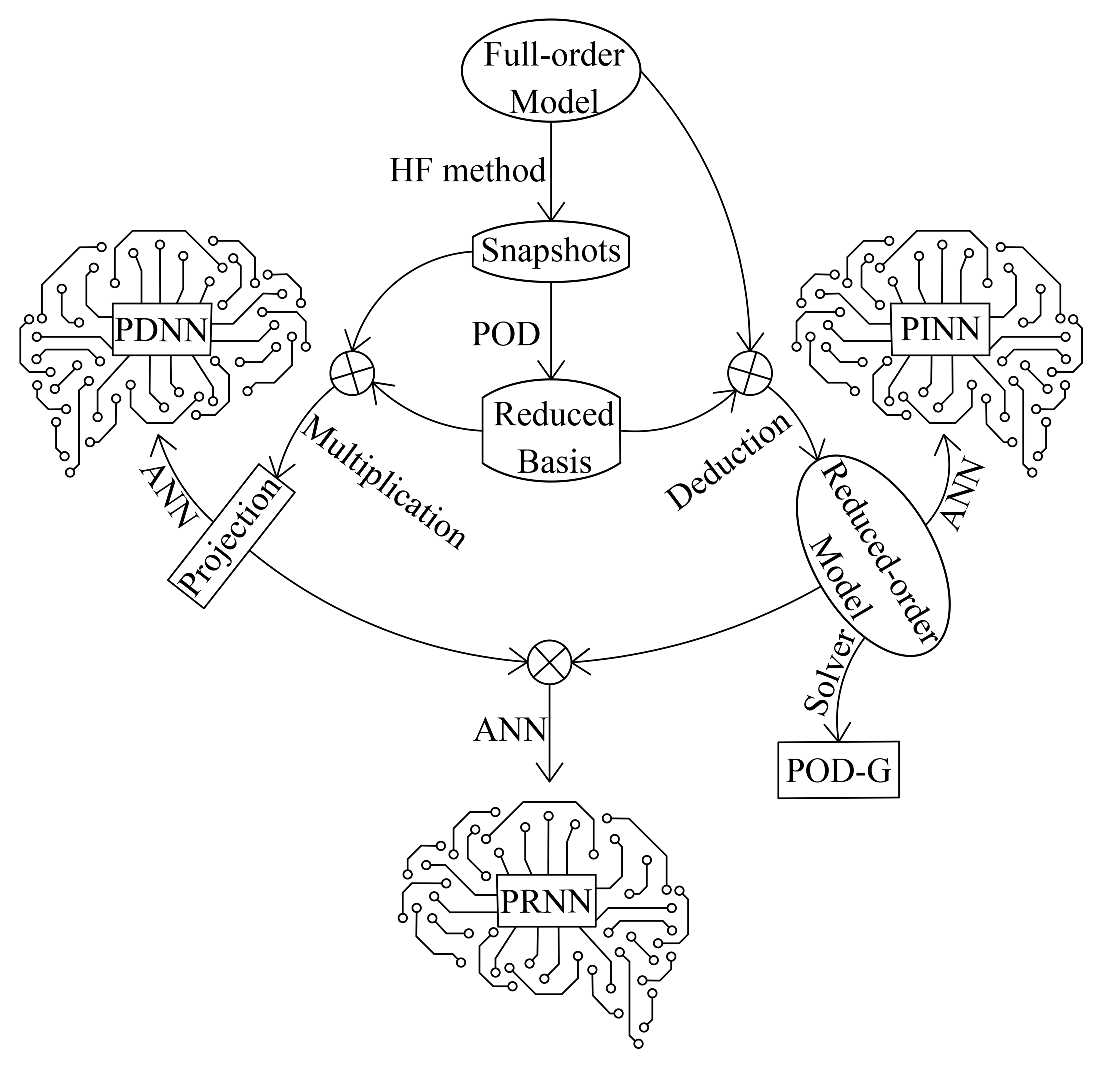
\includegraphics[width=12cm]{../fig/RelationshipChart.pdf}
\caption{Relationship among the projection-driven neural network (PDNN), physics-informed network (PINN) and physics-reinforced neural network (PRNN).}
\label{fig_relationship}
\end{figure}

In the next subsections, we first briefly introduce the basic idea of artificial neural networks. Then we will start from the projection-driven neural networks proposed by Jan \cite{hesthaven2018non}. After that, the proposed physics-inform neural network and physics-reinforced neural network will be detailed.


\subsection{Artificial neural network (ANN) }
For an arbitrary target function, ANN is a powerful nonlinear approximator constituted of a linear combination of some nonlinear functions. Generally, ANN contains $L$ hidden layers besides input and output layers,  the $i$th layer equipped with $n_l$ neurons, where $l=0,1,..L,L+1$ denotes the input layer, 1st hidden layer,..., $L$th hidden layer and the output layer, respectively. ANN can be expressed as a nonlinear function $\mathcal{O}: \mathbf{R}^{n_0} \mapsto \mathbf{R}^{n_{L+1}}$ of inputs $\mathbf{x}$, comprising a  recursion process
\begin{equation}
\left \{
\begin{aligned}
&\mathcal{O}^{0}   = \mathbf{x} \\
&\mathcal{O}^{l}   = \sigma ^{l} \left( \mathbf{W}^{l} \mathcal{O}^{l-1} + \mathbf{b}^{l}
\right)
\qquad 1 \le l \le L+1
\end{aligned}
\right. ,
\end{equation}
where $\mathcal{O}^{l} \in \mathbf{R}^{n_l}$ is the output of $l$th layer, $n_0$ is the input dimension and $n_{L+1}$ is the output dimension, $\mathbf{W}^{l} \in \mathbf{R}^{n_{l} \times n_{l-1}}$ is the weights, $\mathbf{b}^{l} \in \mathbf{R}^{n_l}$ is the biases and $\sigma ^{l}$ is an element-wise activation function. Usually, the activation function of the output layer is just set as the identification function, namely $\sigma ^{L+1}\left(\mathbf{x}\right)=\mathbf{x}$, while the activation function of all hidden layers are set as a same nonlinear function.

In this work, we simply set the activation function as Swish function \cite{ramachandran2017searching} $ \text{Swish}(x) =x \times \text{sigmoid}(x)$ and use the same number of neurons in each hidden layer, namely $n_1=n_2=,...,=n_L=n_H$ , if not stated otherwise. For a specific ANN architecture ($L$ the network depth and $n_H$ the network width), the weights and biases of ANN are trained to minimize the discrepancy between ANN outputs and targets for the given inputs, where the discrepancy is metricized by a scalar loss function. Thus the training of ANN is essentially an single-objective minimization problem
\begin{equation}
\mathop {\arg \;\min }\limits_{{\mathbf{W,b}}} \;
loss\left( {\mathcal{O}\left(\mathbf{x}\right),\mathcal{O}_\text{target} \left(\mathbf{x}\right)} \right)
.
\end{equation}
However, optimizing the minimization problem is not trivial. As for approximating a complex nonlinear target function with high dimensional inputs/outputs, an ANN of large depth and width is always necessary, resulting in a much larger size of independent variables in $\mathbf{W,b}$, where $\mathbf{W}=\{\mathbf{W}_i\}_{i=1}^{L+1}$ and $\mathbf{b}=\{\mathbf{b}_i\}_{i=1}^{L+1}$. Thus many numerical issues will emerge, among which local minima and overfitting traps are the most common cases. Luckily, many training techniques have been developed in last decades, such as Mini-Batch method to relieve local minima trap and regulation method to relieve overfitting trap.

\subsection{Customized networks}
%To get a good mapping form parameter $\pmb{\mu} \in \mathcal{P}$ to the projection of snapshot $\pmb{\phi}_h \in \mathbf{R}^{N}$ in reduced sapce, a ANN is built and trained based on reduced basis.

Some preparation need to be made before introducing the customized networks. Recall that the snapshot set $\pmb {\Phi}_{\mathcal{P}_M}=\{\pmb{\phi}_h(\pmb{\mu}_1), \pmb{\phi}_h(\pmb{\mu}_2),...,\pmb{\phi}_h(\pmb{\mu}_M)\}  \in \mathbf{R}^{N \times M}$ corresponding with the parameter set $\mathcal{P}_M=\{\pmb{\mu}_1, \pmb{\mu}_2,...,\pmb{\mu}_M\} \subset \mathcal{P}$ is employed to extract the reduced basis $\mathbf{V}$ , according to Section \ref{sec_ROM}. Due to the orthogonality of $\mathbf{V}$, the projection coefficient of each snapshot on the reduced space is derived by left multiplying Eq. (\ref{eq_projection}) with $\mathbf{V}^T$, namely
\begin{equation}
\begin{aligned}
\pmb{\alpha}  &   =    \mathbf{V}^T (\pmb{\phi}_h -\tilde{\phi} - \pmb{\epsilon}) \\
              &\approx \mathbf{V}^T (\pmb{\phi}_h -\tilde{\phi})
.
\end{aligned}
\label{eq_RBCoefficients}
\end{equation}

All the parameters in $\mathcal{P}_M$ along with the projections of their corresponding snapshots, denoted by $\mathcal{D}_{Pr}=\left\{\left(\pmb{\mu}_i, \left. {\pmb{\alpha}} \right|_{\pmb{\mu}=\pmb{\mu}_i}
\right) \right\}_{i=1}^{M}$,  is collected as an input-output data set. As the projection is the best approximation to the snapshot with only the projection error, the data set $\mathcal{D}_{Pr}$ is the best choice for training an ANN.

As ANN is sensitive to the difference in dimensional scale of inputs/outputs \cite{ioffe2015batch},
the data set $\mathcal{D}_{Pr}$ needs to be further normalized before feeding it into the ANN. For inputs, namely $\pmb{\mu} \in \mathcal{P}$, as the range of the parameter space is always acknowledged, the minimal and maximal of the parameter space can be utilized to scale the inputs to $[-1,1]^{n_0}$, which is formulated as follows
\begin{equation}
\tilde{\pmb{\mu}}(\pmb{\mu}) =
\frac
{{\pmb{\mu}}- ( {\pmb{\mu}}_{\max} +{\pmb{\mu}}_{\min} )/2}
{             ( {\pmb{\mu}}_{\max} -{\pmb{\mu}}_{\min} )/2}
.
\label{eq_InputsNormalization}
\end{equation}
We note that the division in Eq. (\ref{eq_InputsNormalization}) denotes an element-wise operation, and it also applies in the following.
As for the outputs, there is not an prior range of the output, however. We turn to a statistical method to do the normalization with an assumption that the outputs satisfy the Gaussian distribution. To this end, the standard derivation $\pmb{\Theta}$ and mean $\overline {\pmb{\alpha}}$ of outputs are calculated dimension by dimesion, and then the outputs are normalized as follows
\begin{equation}
\tilde{\pmb{\alpha}}(\pmb{\alpha}) =
\frac
{{\pmb{\alpha}}- \overline {\pmb{\alpha}}}
{     \pmb{\Theta}         }
.
\end{equation}
We wrap the normalisation of inputs/ouputs into the ANN as follows
\begin{equation}
\tilde{\mathcal{O}}\left(\pmb{\mu}\right)
 =
{\mathcal{O}}\left(\mathbf{ \tilde{\pmb{\mu}}(\pmb{\mu}) }\right)
\otimes
\pmb{\Theta} + \overline {\pmb{\alpha}}
.
\end{equation}
Thus, the inputs and outputs of the wrapped network  $\tilde{\cal{O}}(\bullet)$ will be physical variables, while the inputs and outputs of the original network $\mathcal{O}(\bullet)$  will be normalized variables.

\subsubsection{Projection-driven neural network(PDNN)}
The data set $\mathcal{D}_{Pr}$ is used directly to train the network to avoid building the reduced-order model. The data set $\mathcal{D}_{Pr}$ is randomly split into two parts: train set $\mathcal{D}_{Pr}^{tr}$ and validation set $\mathcal{D}_{Pr}^{va}$. The famous Adam  stochastic  optimizer \cite{kingma2014adam} is employed to train the network. The ratio between the size of $\mathcal{D}_{\rm{POD}}^{tr}$ and $\mathcal{D}_{Pr}$  is set as 0.7. The loss function is defined as the mean square error between network outputs and targets scaled with the standard derivation $\Theta$, namely
\begin{equation}
loss_{\rm{PDNN}} = \frac{1}{N_{\cal D}}
{{\sum\limits_{\pmb\mu ,\pmb\alpha  \in {\cal D}} {{{\left\| {\frac{\left( {\widetilde {\cal O}\left( {\pmb\mu ;{\bf{W}},{\bf{b}}} \right) - \pmb{\alpha} } \right)} {\pmb{\Theta}} } \right\|}^2}} }},
\end{equation}
where $\cal D$ is the chosen data set of size $N_{\cal D}$, which can be the train set $\mathcal{D}_{Pr}^{tr}$ or the validation set $\mathcal{D}_{Pr}^{va}$.

In real applications, we are not expected to generate too many snapshots, since the full-order model is always expensive. Thus the data set size $\mathcal{D}_{Pr}$ is always very small, so the training of the network will get trapped into overfitting problem. To prevent overfitting, first the $L_2$ regulation technique is employed by penalizing the loss of the train set with the weights $\bf{W}$
\begin{equation}
\widetilde{loss}_{\rm{PDNN}}
 = loss_{\rm{PDNN}}
  + \eta {\left\| { \mathbf{W} } \right\|}^2,
\end{equation}
where $\eta$ is the decay weight.
Besides, we adopt the early stopping criterion: training will be immediately stopped only if the validation loss keeps increasing over $K_{early}$ epoches. In what remains, $\eta=10^{-4}$ and $K_{\rm{early}}=6$ are employed.

\subsubsection{Physics-informed neural network(PINN)}
Due to the limited number of available snapshots, it is always difficult to train a good network with Projection-driven neural network. Luckily, we have the reduced-order model, an another choice for training an ANN. Given the reduced-order model, ANN outputs need not explicitly approximate some given targets, but just satisfy the reduced-order model. In this way, no target is needed, and thus we have unlimited training data. By Latin hypercube sampling in parameter space, we generate the data set $\mathcal{D}_{Resi}=\{ \pmb{\mu}_i\}_{i=1}^{M_{Resi}}$, containing $M_{Resi}$ residual points in parameter space. The loss function is defined as follows
\begin{equation}
{loss}_{\rm{PINN}} = \frac{1}{N_{\cal D}}
{{\sum\limits_{\pmb\mu  \in {\cal D}}
{ \left\|
ROM \left(\widetilde {\cal O}\left( {\pmb\mu ;{\bf{W}},{\bf{b}}} \right) \right)
\right \|^2}
}},
\end{equation}
where $ROM(\pmb{\alpha})=\mathbf{V}^T
\left(
 \mathbf{L} \mathbf{V} \pmb{\alpha}
+ g         \left( \mathbf{V} \pmb{\alpha} \right)
+\mathbf{C}
\right)$
is the reduced-order model defined in Eq. (\ref{eq_Galerkin}).
As we have unlimited training data, there is no problem of overfitting and thus no need of validation data set.  The bottleneck of training the physics-informed neural network is how to handle the local minima trap. Here, we adopt the mini-batch training method, where the data set are shuffled and randomly into serval non-overlap subsets in each epoch. With each subset, the weights and biases will be updated by optimizer. The mini-batch training method can effectively avoid local minima trap and has enjoyed great success in lots of applications.

\subsubsection{Physics-reinforced neural network(PRNN)}
\label{PRNN}
Physics-informed neural network(PINN) seems an perfect potential in predicting projection coefficients. But numerical experiments show that  the accuracy of the physics-informed neural network sometimes is not that good, even if the the corresponding loss drops down to a very low level. The underlying reason comes from that the large scale difference of different RB modes.
First, the RB mode with smaller index will be more dominant to the residual of the reduced-order model. Second, the training of network cannot work like a deterministic nonlinear solver, and it can only reduce the loss to a moderate level. Thus, the reduced-order model cannot be well-solved thorough training network. As a result, the optimizer tends to neglect the relatively unimportant modes, namely the high-index modes.

To address this problem, we add the acknowledged data set ${\cal {D}}_{Pr}$ into the loss function of PINN. Although the projection coefficients in ${\cal {D}}_{Pr}$  are always not the solutions of the reduced-order model, the corresponding projections are closer to the snapshots and thus full-order model. Besides, the projection coefficients is calculated directly according to Eq. \ref{eq_RBCoefficients}, and it has no problem of domination for different modes. Therefore, the projection coefficients can be used to provide more physical information into the network training. Thus we name this method as physics-reinforced neural network. The loss function is defined as the weighted sum of those of PDNN and PINN, namely
\begin{equation}
{loss}_{\rm{PRNN}} =
\left. {{loss}_{\rm{PDNN}}} \right|_{{\cal{D}} = {\cal {D}}_{Pr} }
+
w \times \left. {{loss}_{\rm{PINN}}} \right|_{{\cal D} = {\cal D}_{Resi }},
\label{eq_lossPRNN}
\end{equation}
where $w$ is a specific weight balancing projection and reduced-order model. In this work, we find that simply setting $w=1$ will produces a good result.  When training the network, the two data sets are treated separately. As for projection data set ${\cal D}_{Pr}$, it is more accurate but its size is very small, so we continue to use full batch. As for residual data set ${\cal D}_{Pr}$, it is less accurate but its size is very large, and we use mini-batch method for each updating of the network.

\section{Numerical results and discussion}
In this section,
we will discuss the application of PDNN, PINN and PRNN methods to the following parameterized PDEs, namely the one-dimensional Burges' equation, two-dimensional lid driven flow and natural convection flow.
The one-dimensional case are designed with an artificial solution with a zero-value boundary condition, intended for testing the prediction accuracy of the three networks and also study the influence of several factors. Their prediction accuracy are further discussed the two realistic flow problems, where geometry parameters and common boundary conditions (Dirichlet and Neumann) are included.

Besides, for comparison of accuracy, the results of two analytical methods are also considered:
\begin{enumerate}[(1)]
\item \textbf{Projection}: Projection of high-fidelity solution onto reduced basis;
\item \textbf{POD-G}: The solution of the reduced-order model.
\end{enumerate}
As the PDNN is trained with the projection coefficients of high-fidelity solutions, the PDNN targets the accuracy of the Projection. The PINN is trained to meet the reduced-order model, the PINN targets the accuracy of the POD-G. The PRNN can be viewed as a blending of the PDNN and PINN, and thus its accuracy is expected to fall somewhere between those of the Projection and POD-G.

To assess the online accuracy of these methods, the following metrics are defined in the sense of mean relative Euclidean distance.
\begin{enumerate}[(1)]
\item the average relative error of  projections
\begin{equation}
\varepsilon_{\rm{Proj}}
=\frac{1}{N_{{\cal D}_{te}}}
\sum\limits_{\pmb\mu ,\pmb{\phi}_h  \in {{\cal D}_{te}}}{
\frac{\left\| \pmb{\phi}_h - \tilde{\phi} -\mathbf{V}\mathbf{V}^T \left( \pmb{\phi}_h - \tilde{\phi} \right)  \right\|}
{\left\| \pmb{\phi}_h  - \tilde{\phi} \right\|}
};
\end{equation}

\item the average relative error of POD-G solutions
\begin{equation}
\varepsilon_{\bullet}
=\frac{1}{N_{{\cal D}_{te}}}
\sum\limits_{\pmb\mu ,\pmb{\phi}_h  \in {{\cal D}_{te}}}{
\frac{\left\| \pmb{\phi}_h- \tilde{\phi}-\mathbf{V}\pmb{\alpha}_{\bullet}\left( \pmb{\mu}\right)
\right\|}
{\left\| \pmb{\phi}_h - \tilde{\phi} \right\|}
}.
\end{equation}

\end{enumerate}
where ${{\cal D}_{te}}=\{\pmb{\mu}_i, \pmb{\phi}_h(\pmb{\mu}_i)\}_{i=1}^{N_{{\cal D}_{te}}}$ is the test data set of size ${{\cal D}_{te}}$, the subscript "$\bullet$" is used to take the place of "POD-G","PDNN","PINN" and "PRNN", respectively. Thus, $\pmb{\alpha}_{\bullet}\left( \pmb{\mu}\right)$ is the solution calculated from the corresponding method.

Note that the Projection, POD-G, PDNN, PINN and PRNN methods are all coded in Python. The networks built are all under the framework of Pytorch. The training of networks are all  implemented on two GUPs (NVIDIA Quadro GP100) of a server class station. To solve the reduced-order model directly for the POD-G method, the nonlinear solver "linalg.solve" in  Numpy library is employed. We refer the reader to the repository \footnote{available at \url{https://github.com/cwq2016/POD-PINN}} for further details of the code. For different data set as discussed above, we employ the specific sampling methods in parameter space: for building the RB, we adopt the Sobol sequences, a quasi-random low-discrepancy sequences; For choosing residual points, we use the Latin hypercube sampling; For generating test data set, we employ uniform tensor-product grid.


\subsection{Burgers' equation}
In this subsection, to validate the proposed methods, we consider the  following one-dimensional parameterized Burges' equation
\begin{equation}
\left\{
\begin{aligned}
	 &\phi(x;\pmb{\mu}) \cdot \nabla \phi(x;\pmb{\mu}) -  \Delta \phi(x;\pmb{\mu})= s(x;\pmb{\mu})  \qquad -1 \le x \le 1\\
	 &\phi\left ( x= \pm1; \pmb {\mu} \right ) = 0
\end{aligned}\right.
,
\end{equation}
where $\pmb{\mu} =(\mu_1, \mu_2) \in [1,10] \times [1,10]$ and $s(x;\pmb{\mu})$ is the source term defined so that the exact solution satisfies
\begin{equation}
	\phi(x; \pmb{\mu}) = (1+\mu_1 x)\sin(-\mu_2 x/3) (x^2-1) .
\end{equation}
The solution at the two end points are simply set zero to avoid the influence of boundary conditions. The problem is solved with Chebyshev pseudospectral (PS) method with $N_p+1$=128+1 Chebyshev Gauss-Lobatto points.


We are interested in the prediction accuracy of the Projection, POD-G, PDNN, PINN and PRNN methods. The accuracy of Projection and POD-G is only determined by two factors, namely the sample size $N_s$ for building reduced basis (RB) and and the number of chosen modes $m$, provided that the nonlinear solver for the POD-G is accurate enough. Here we term the two factors as essential factors.
Besides the two factors, the neural networks,  namely the PDNN, PINN and PRNN,  are also determined by network architecture, the number of residual points, and so on. To study the influence of these factors, we resort to the control variates method. Some base values are set for these factors, namely sample size is $N_s=80$, the number of chosen modes is picked from the set $\{2,3,...,9\}$,  network architecture is $L=3$ and $n_H=20$, the number of residual points is $N_{Resi}=5000$. To test the prediction accuracy, a test data set of size $101 \times 101=10201$ is generated on a tensor-product parameter grid $\{1+ 0.09i\}_{i=0}^{i=100} \times \{1+ 0.09i\}_{i=0}^{i=100}$. The dense test grid will guarantee the reliability of the prediction accuracy. As for the training of networks, we use the same following hyperparameters: 20000 epoches, 10 batches with each batch of size $N_{Resi}/10$, leaning rate initialized as 0.01 and decaying by 96\% every 200 epoches.

We first study the influence of the sample size. Fig. \ref{fig_1DBurgesSingularValues_80}, presents the singular value distribution for the sample number $N_s=80$. It is shown that the singular value decays quickly, implying that  a small number of RB modes is enough for representing the dynamic of the problem. Meanwhile, the number of samples for building the necessary RB modes can also be largely reduced. Thus, for comparison, $N_{s}=10$ and 320 random parameter samples are independently generated with Sobol sequences, and also their corresponding snapshots are calculated. The five methods are applied to the problem after the RB is built for $N_{s}=10$, 80 and 320, respectively. The prediction accuracy is shown in Fig. \ref{fig_1DBurgesErrorComparsion_SampleNum}. It is shown that the Projection enjoys a better accuracy compared with the POD-G, but their discrepancy is very small. The pojection/POD-G improves just a little for sample number $N_s$ increasing from 10 to 80, and almost stagnates from $N_s=80$ to 320. Thus, sample number $N_s=10$ is enough for capture the main dynamic of the problem. The networks perform quite differently. The accuracy of PDNN is far lower than that of PINN and PRNN. Even with the increase of sample number, the accuracy of PDNN can improve by one order of magnitude, but the error curves fluctuate intensively especially for larger $m$. On the contrary, both PINN and PRNN perform much better, they almost keep pace with POD-G for smaller $m$. As $m \ge 6$, the PINN performs a little better than the PRNN, but their error level both come to a saturation and cannot further drop down. The reason for the saturation is that both the PINN and PRNN can only reduce their loss function down to a level of $10^{-6}$ for this problem rather than zero or machine zero level. Thus the high-index modes of little importance are neglected by the networks.  The PINN performs a little better than the PRNN, which is opponent with our inference in Section \ref{PRNN}. The reason is that two-fold: first, the PINN performs near the POD-G;  second, the POD-G is very close to the Projection. And the priority of the PRNN will be revealed when their discrepancy increases, as shown for the more complex problems in next two subsections.
\begin{figure}[!ht]
    \centering
    \subfigure{
        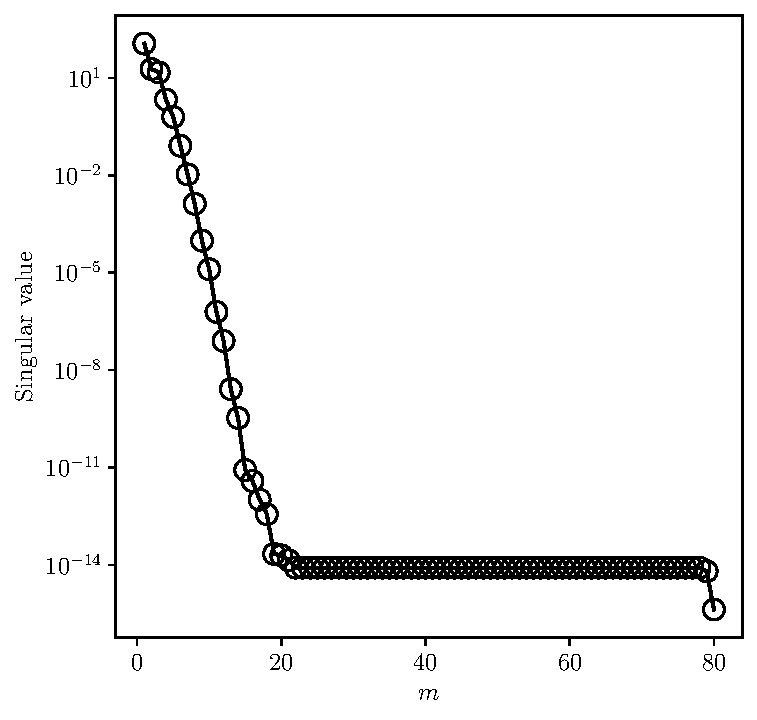
\includegraphics[width=7cm]{../../pythonNN/1DBurges/fig/SingularValues_80.pdf}
        \label{fig_1DBurgesSingularValues_80}
    }
    \subfigure{
        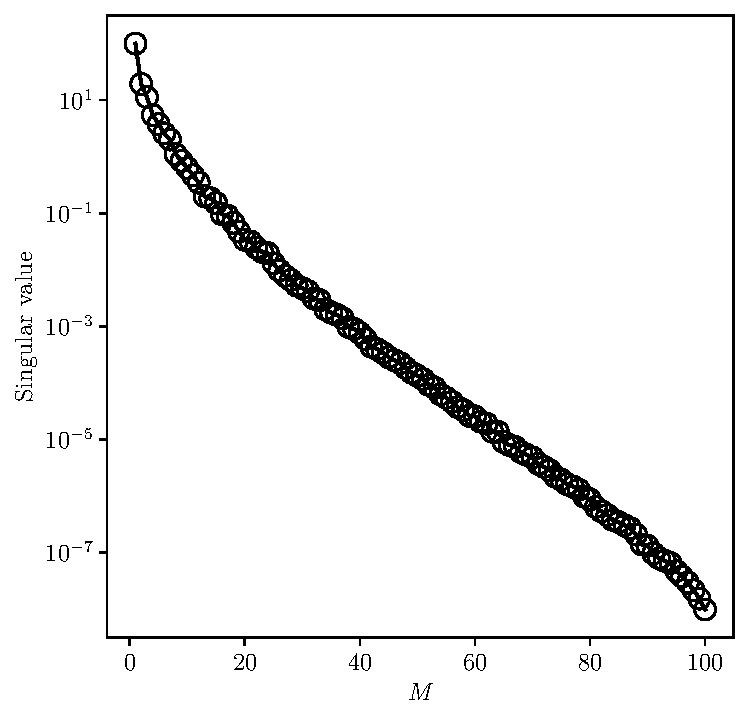
\includegraphics[width=7cm]{../../pythonNN/2DLidDriven/fig/SingularValues_100.pdf}
        \label{fig_2DLidDrivenSingularValues}
    }

    \subfigure{
        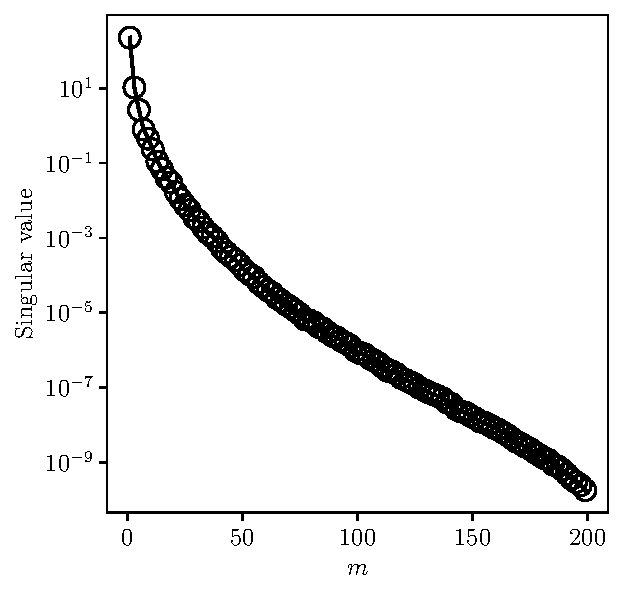
\includegraphics[width=7cm]{../../pythonNN/2DNaturalConvection/fig/SingularValues_200.pdf}
        \label{fig_2DNaturalConvectionSingularValues}
    }
\caption{Singular value distribution for (a) 1D Burges' equation with 80 snapshots, (b) 2D lid -driven flow with 100 snapshots and (c) 2D Natural convection with 200 snapshots.}
\end{figure}


%\begin{figure}[!ht]
%  \centering
%  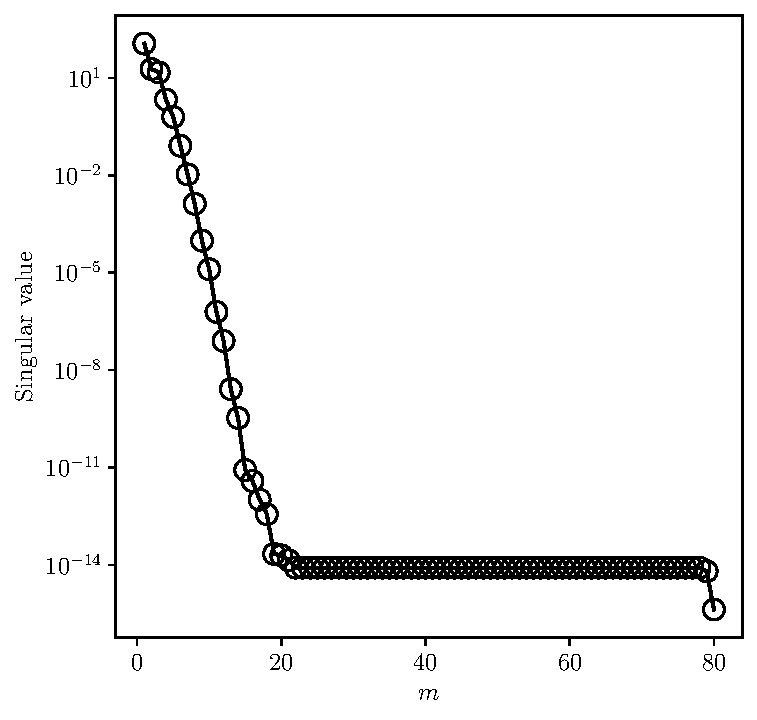
\includegraphics[width=9cm]{../../pythonNN/1DBurges/fig/SingularValues_80.pdf}
%\caption{Singular value distribution of 80 snapshots for 1D Burges' equation}
%\label{fig_1DBurgesSingularValues_80}
%\end{figure}

\begin{figure}[!ht]
  \centering
  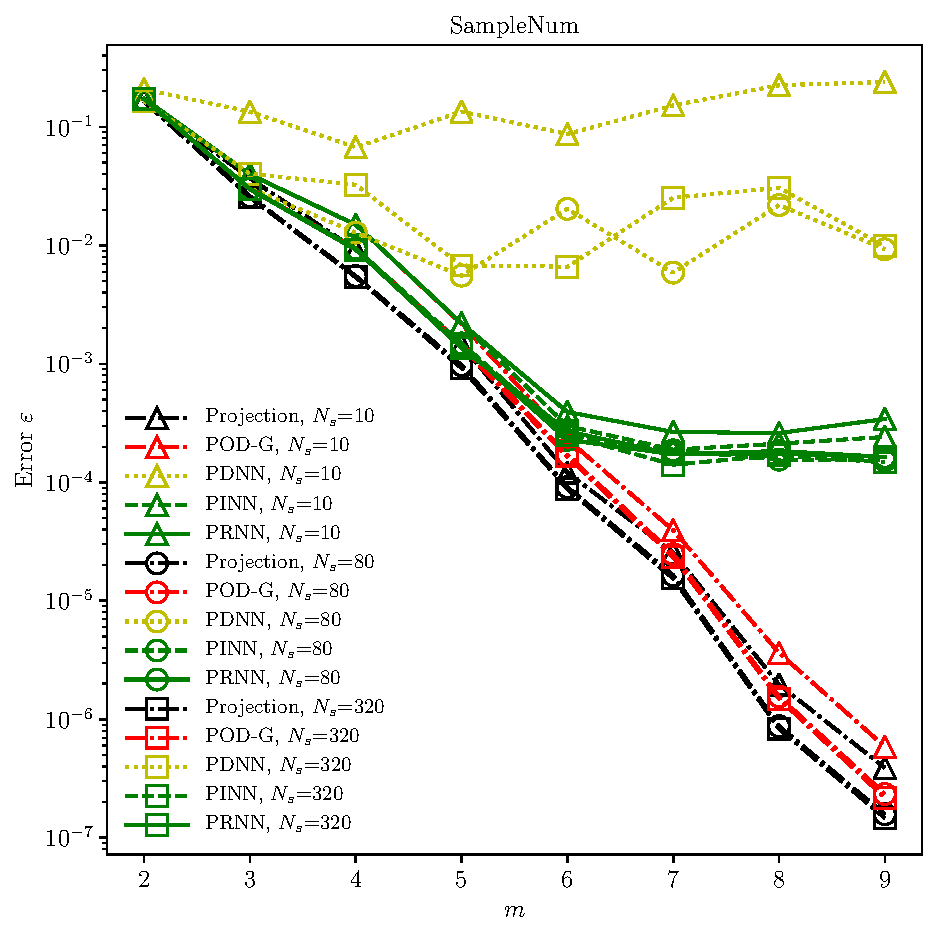
\includegraphics[width=12cm]{../../pythonNN/1DBurges/fig/ErrorComparsion_SampleNum.pdf}
\caption{The prediction accuracy of the Projection, POD-G, PDNN, PINN and PRNN methods for the number of snapshots $N_s$=10, 80 and 320, respectively.}
\label{fig_1DBurgesErrorComparsion_SampleNum}
\end{figure}


To further study the influence of network architecture on the prediction accuracy of the three networks, we change network width to $n_H=10$ and $n_H=30$, respectively, while keeping network depth $L=3$ fixed. The results are shown in Fig. \ref{fig_1DBurgesErrorComparsion_Netsize}. It is shown that the PDNN can not gain an obvious improvement of accuracy with the increase of $n_H$, or even get rid of the fluctuation, resulting from the overfitting trap. On the contrary, the PINN and PRNN show a much better tendency. Their prediction accuracy increases with $n_H$ but tends to saturate for a larger $n_H$. This is in accordance with the situation that the approximation capability of the network increases and gradually saturate with the increase of network size.

As there are unlimited residual points available for training both the PINN and PRNN, we are interested in how the number of residual points influence the prediction accuracy. In addition to $N_{Resi}=5000$, the numbers of residual points $N_{Resi}=1250$, $2500$ and $10000$ are considered, and the results are shown in Fig. \ref{fig_1DBurgesErrorComparsion_NResi}. The influence of the number of residual points is similar with that of network architecture. That is to say, the prediction accuracy increases with the number of residual points $N_{Resi}$, but it will reach a saturation after some critical $N_{Resi}$.

Besides, the further confirmation of the reliability of PRNN is shown in Fig. \ref{fig_1DBurgesResultComparsion}, offering a good agreement between the Chebyshev pseudospectral method and PRNN for some specific parameters.

\begin{figure}[!ht]
  \centering
  \includegraphics[width=9cm]{../../pythonNN/1DBurges/fig/ErrorComparsion_Netsize.pdf}
\caption{The prediction accuracy of the Projection, POD-G, PDNN, PINN and PRNN methods. The network width is set $n_H=10$, 20 and 30, respectively.}
\label{fig_1DBurgesErrorComparsion_Netsize}
\end{figure}

\begin{figure}[!ht]
  \centering
  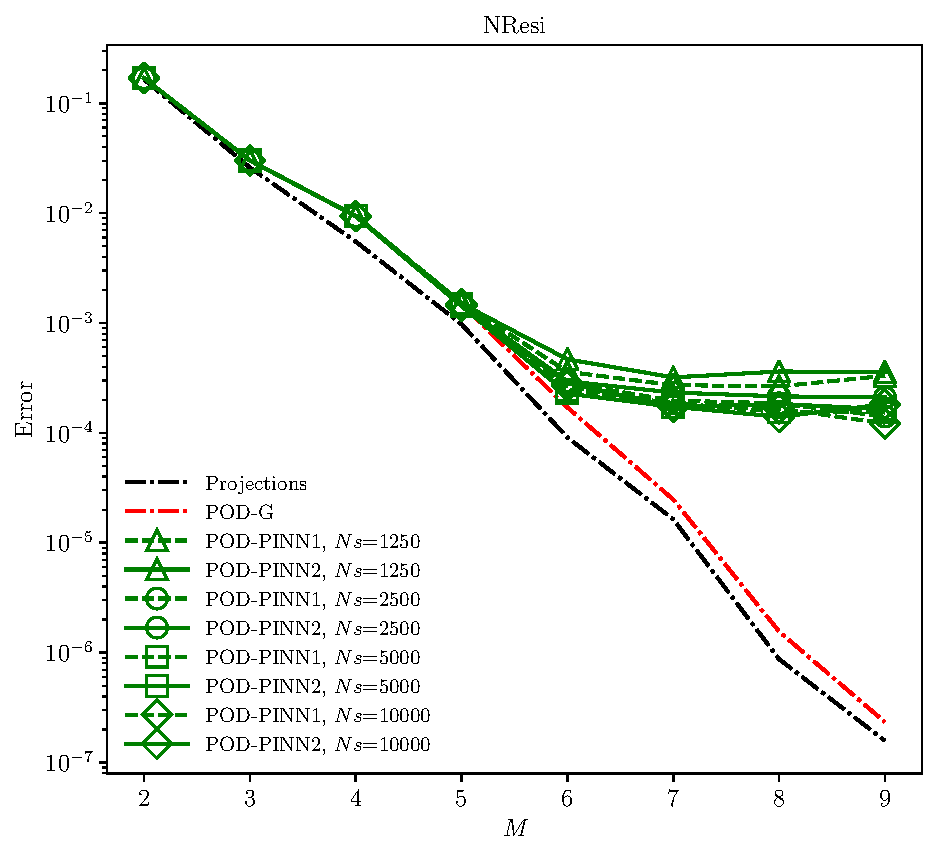
\includegraphics[width=9cm]{../../pythonNN/1DBurges/fig/ErrorComparsion_NResi.pdf}
\caption{The prediction accuracy of the Projection, POD-G, PINN and PRNN methods. $N_{Resi}$=1250, 2500, 5000, 10000 residual points are chosen for training the PINN and PRNN.}
\label{fig_1DBurgesErrorComparsion_NResi}
\end{figure}

\begin{figure}[!ht]
  \centering
  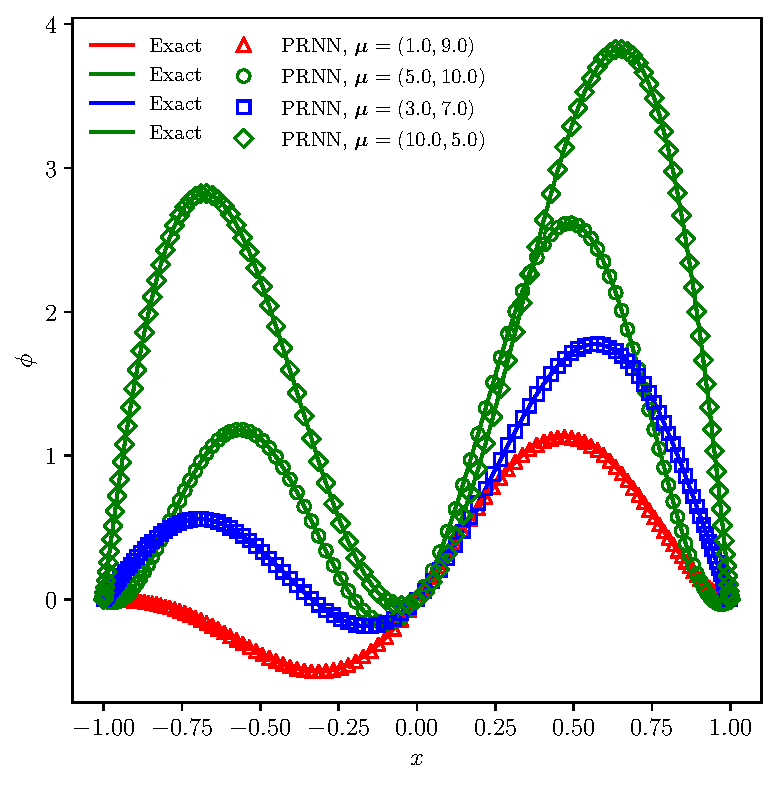
\includegraphics[width=9cm]{../../pythonNN/1DBurges/fig/ResultComparsion.pdf}
\caption{The comparison between the Chebyshev pseudospectral (PS) and the PRNN solutions for four specific parameters. The results of the PRNN are obtained via employing the $m$=9 modes extracted from 10 snapshot and a network of $L$=3 and $n_H$=20 architecture trained with 5000 residual points.}
\label{fig_1DBurgesResultComparsion}
\end{figure}


\subsection{Lid-driven flow}
The lid-driven flow is considered for testing the prediction accuracy of the proposed methods in handling realistic problem.
The flow is governed by the following non-dimensional incompressible Navier-Stokes equations
\begin{equation}
\left \{
\begin{aligned}
\nabla_{\mathbf{x}}  \cdot {\bf{u}} &= 0 \\
\left( {{\bf{u}} \cdot \nabla_{\mathbf{x}} } \right){\bf{u}} &=  - \nabla_{\mathbf{x}} p + \frac{1}{Re}{\nabla_{\mathbf{x}} ^2}{\bf{u}}
\end{aligned}
\right .
,
\label{eq_GoverningEqsLidDriven}
\end{equation}
where $\mathbf{u}=(u,v)$ is the dimensionless velocity in Cartesian coordinate $\mathbf{x}=(x,y)$, $p$ is the pressure, $\nabla$ is the  Hamiltonian operator, $Re$ is the Reynolds number.  The geometry of the problem is dipicted in Fig. \ref{fig_geometry}(a), which is affected by  the inclining angle $\theta$ of the left and right side walls. The Reynolds number and the inclining angle are the parameter $\pmb {\mu} $ controlling the problem. In order to address the variable geometry, the physical domain  is mapped to an square domain $[-1,1]^2$. The mapping $\mathcal{X}$ from the physical domain $\mathbf{x} \in \Omega\left(\pmb{\mu}\right)$ to the computation domain $\pmb{ \xi}=(\xi_1, \xi_2) \in [-1,1]^2$  and its inverse $\mathcal{X}^{-1}$ are defined as follows:
\begin{equation}
\mathcal{X}:
\left \{
\begin{aligned}
x &= 1/2 \xi_1 + 1/2 \xi_2 \cos(\theta)\\
y &= 1/2 \xi_2 \sin(\theta)
\end{aligned}
\right .
\qquad
\rightleftharpoons
\qquad
\mathcal{X}^{-1}:
\left \{
\begin{aligned}
\xi_1 &= 2(x-y \cot(\theta))\\
\xi_2 &= 2y/\sin(\theta)
\end{aligned}
\right . .
\end{equation}
Thus, we have the Jacobin matrix of the mapping
\begin{equation}
\mathbf{J} = \frac{\partial \mathbf{x}}{\partial \pmb{\xi}}
           =
\begin{bmatrix}
 &2             & 0\\
 &-2\cot(\theta)&2/\sin(\theta)
\end{bmatrix}.
\label{eq_JacLidDriven}
\end{equation}
Substituting Eq. \ref{eq_JacLidDriven} into Eq. \ref {eq_GoverningEqsLidDriven}, we have the governing equation in computational space:
\begin{equation}
\left \{
\begin{aligned}
\left(\mathbf{J}^{-1} \nabla_{\pmb {\xi}}\right)  \cdot {\bf{u}} &= 0 \\
\left( {{\bf{u}} \cdot \left(\mathbf{J}^{-1} \nabla_{\pmb {\xi}}\right) } \right){\bf{u}} &=  - \left(\mathbf{J}^{-1} \nabla_{\pmb {\xi}}\right) p + \frac{1}{Re}{\left(\mathbf{J}^{-1} \nabla_{\pmb {\xi}}\right) ^2}{\bf{u}}
\end{aligned}
\right .
.
\label{eq_GoverningEqsCompLidDriven}
\end{equation}


\begin{figure}[!ht]
    \centering
    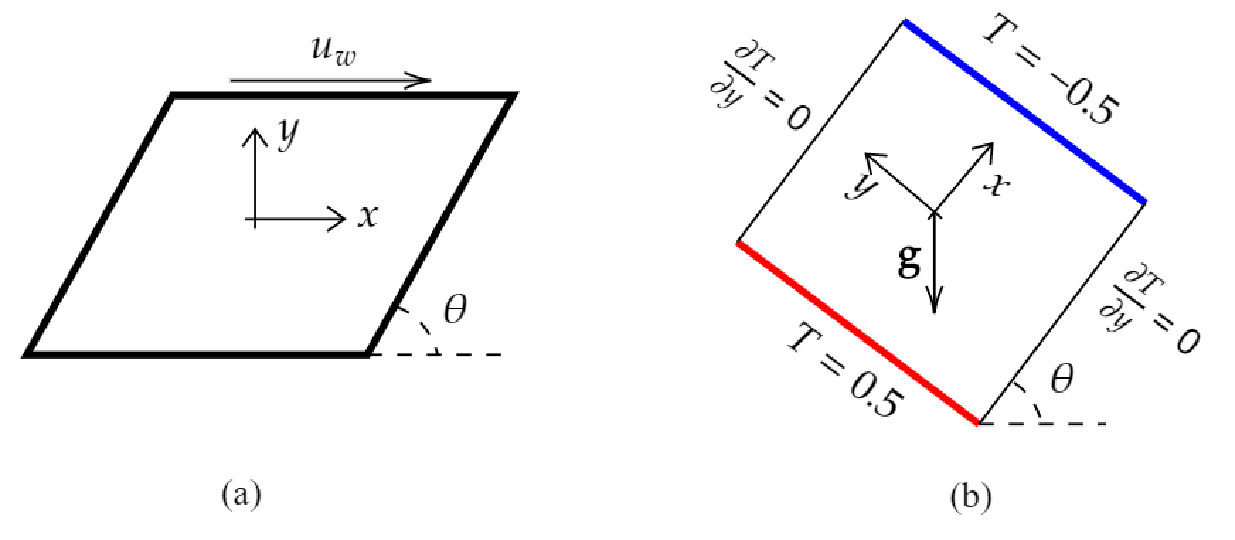
\includegraphics[width=10cm]{..//fig/geometry.pdf}
    \caption{The geometry and boundary conditions for (a) Lid-Driven flow and (b) Natural convection in enclosure.}
    \label{fig_geometry}
\end{figure}


The flow is driven by the top moving wall. All the other three sides are all no-slip walls. Eq. (\ref{eq_GoverningEqsCompLidDriven}) is discritized by the Chebyshev pseudospectral method with a tensor-product grid of $49 \times 49$.
For this problem, it is crucial to address the well-known difficulty of the corner singularity, resulting from the discontinuous horizontal velocity at the two top corners. In this work, to remove the singularity, the velocity of top wall is specified as
\begin{equation}
u_W = (1+\xi_1)^2(1-\xi_1)^2.
\end{equation}
as adopted in references \cite{shen1991hopf, pinelli1994chebyshev, phillips1993treatment}. The $IP_{N}-IP_{N-2}$ method \cite{zhang2010explicit, peyret2013spectral} is employed to remove the spurious modes of pressure.
Besides, the artificial compressibility method \cite{clausen2013entropically} is employed to address the coupling  of velocity field and pressure by  transforming steady  Eq. (\ref{eq_GoverningEqsCompLidDriven}) into an unsteady one in pseudo time. The derived discrete equation is then solved using an explicit fourth-order four-stage Runge-Kutta integrator in pseudo time.

The parameter space of interest is $\pmb{\mu}=(Re, \theta) \in [100,500] \times [\pi/3, 2\pi/3]$. 100 snapshots of high-fidelity solutions for parameters generated with Sobol sequence are calculated and collected for building the reduced basis, and the corresponding singular value distribution is plotted in Fig. \ref{fig_2DLidDrivenSingularValues}. It is shown that the singular value decays slowly, implying that more modes are required to represent the underlying dynamic. Thus we choose the first $m=5, 10,...,30$ modes, respectively.
The prediction accuracy is assessed on a test data set of size $11 \times 11=121$, generated on a tensor-product parameter grid $\pmb{\mu}=\{100+ 40i\}_{i=0}^{10} \times \{\pi/3+ j\pi/15\}_{j=0}^{10}$.
For the POD-G method solving the reduced-order model, the solving always blows up if it starts from an improper initialization. In this work, for testing the prediction accuracy of the POD-G method, the solving of the reduced-order model for a parameter $\pmb{\mu}$ starts from the projection coefficients of the full-order solution $\pmb{\phi}_h \left( \pmb{\mu} \right)$ on the reduced basis.
Besides, for the sake of comparison, we pick the first 30, 60 snapshots from the 100 snapshots to do the same test. As for the training of networks, we use the same following hyperparameters: network architecture $L$=5 and $n_H$=30, 40000 epoches, batch size 1000, leaning rate initialized as 0.01 and decaying by 96\% every 200 epoches.

The prediction accuracy is shown in Fig. \ref{fig_2DLidDrivenErrorComparsion_SampleNum}. It is shown that the POD-G is far away from the Projection, compared with Fig. \ref{fig_1DBurgesErrorComparsion_SampleNum} for the Burges' equation. Similar convergence tendency features the PINN and PRNN, i.e. the accuracy increases with  smaller $m$ but saturates after a critical value of $m$. However, the priority of the PRNN over PINN is demonstrated. The PINN cannot work well, and the PINN will saturate for $m \ge 15$, even if more snapshots are employed for building the reduced basis. The PRNN performs much better, showing a satisfactory properties.
On one way, the PRNN can achieve an accuracy between the POD-G an Projection for smaller $m$, conforming the blending construction of the loss function in Eq. (\ref{eq_lossPRNN}) of the PRNN; on the other way, the PRNN performs better than PINN, and shows an  expected increase of accuracy with the snapshot number $N_S$. The PDNN enjoys an agreement with the Projection for a smaller $m$, and also an improvement with the increase of $m$. However, it quickly deteriorates after a critical value of $m$. What's more, the accuracy of the PDNN using 100 snapshots is lower than only both the PINN and PRNN using 30 snapshots.

All in all, it can be concluded that the PRNN is much better tan the PINN and PDNN. The further confirmation of the reliability of PRNN is shown in Fig. \ref{fig_2DLidDrivenResultComparsion}, offering a good agreement between the Chebyshev pseudospectral method and PRNN for some specific parameters. We note that the streamlines displayed in Fig. \ref{fig_2DLidDrivenResultComparsion} are derived by solving the following Poisson equation for streamfunction  with an acknowledged velocity field:
\begin{equation}
\left \{
\begin{aligned}
{\nabla_{\mathbf{x}} ^2}{\psi}
 = \frac{\partial u}{\partial y} - \frac{\partial v}{\partial x} \qquad x \in \Omega\\
\psi = 0  \qquad \qquad    x \in \partial \Omega
\end{aligned}
 \right .
 .
\label{eq_Streamfunction}
\end{equation}

%\begin{figure}[!ht]
%  \centering
%  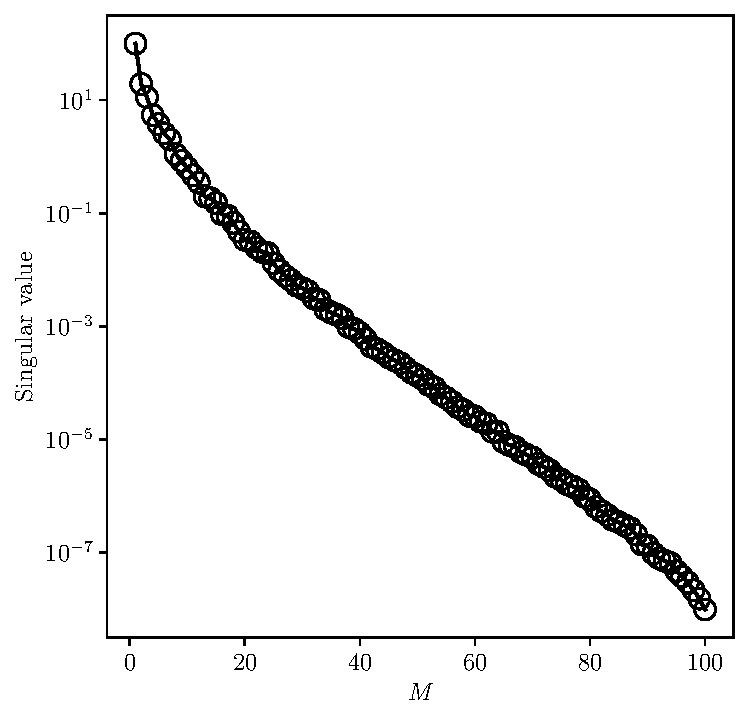
\includegraphics[width=9cm]{../../pythonNN/2DLidDriven/fig/SingularValues_100.pdf}
%\caption{Singular value distribution of 100 snapshots for 2D lid-driven flow}
%\label{fig_2DLidDrivenSingularValues}
%\end{figure}

\begin{figure}[!ht]
  \centering
  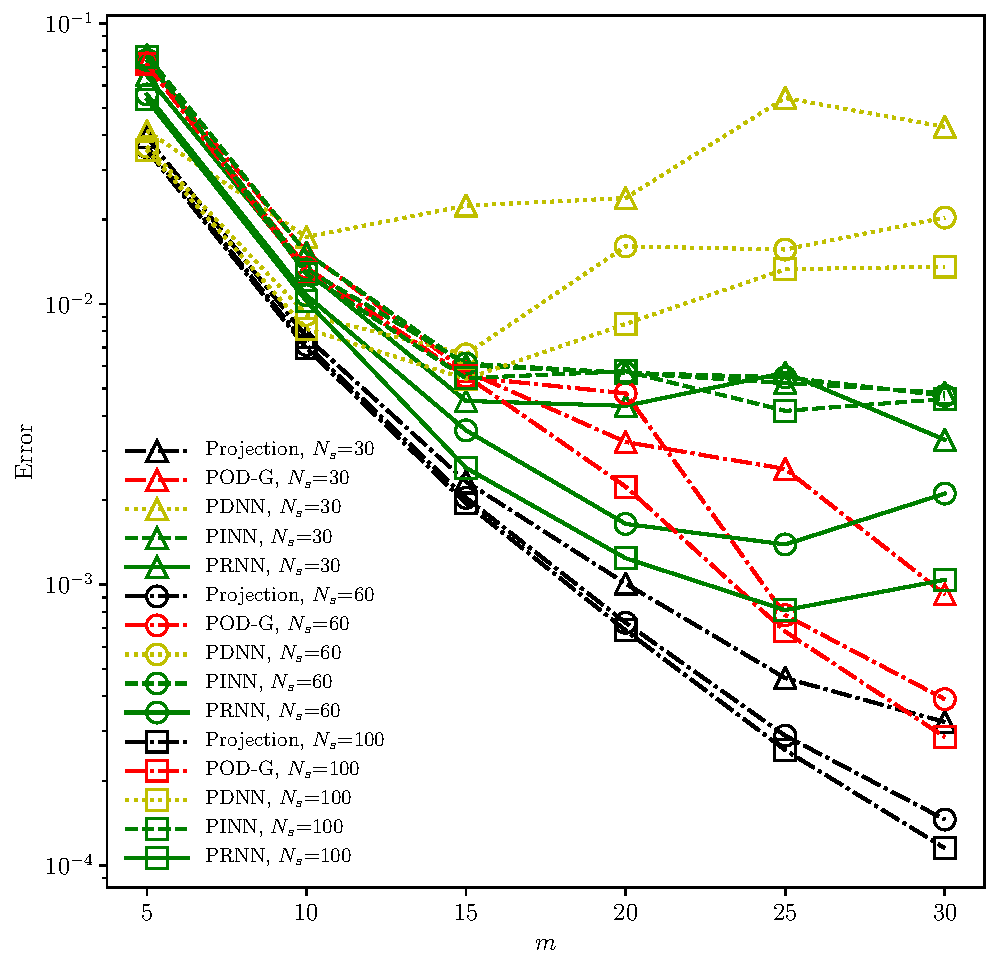
\includegraphics[width=12cm]{../../pythonNN/2DLidDriven/fig/ErrorComparsion_SampleNum.pdf}
\caption{The prediction accuracy of the Projection, POD-G, PDNN, PINN and PRNN methods for 2D lid-driven flow with the number of snapshots $N_s$=30, 60 and 100, respectively.}
\label{fig_2DLidDrivenErrorComparsion_SampleNum}
\end{figure}

\begin{figure}[!ht]
  \centering
  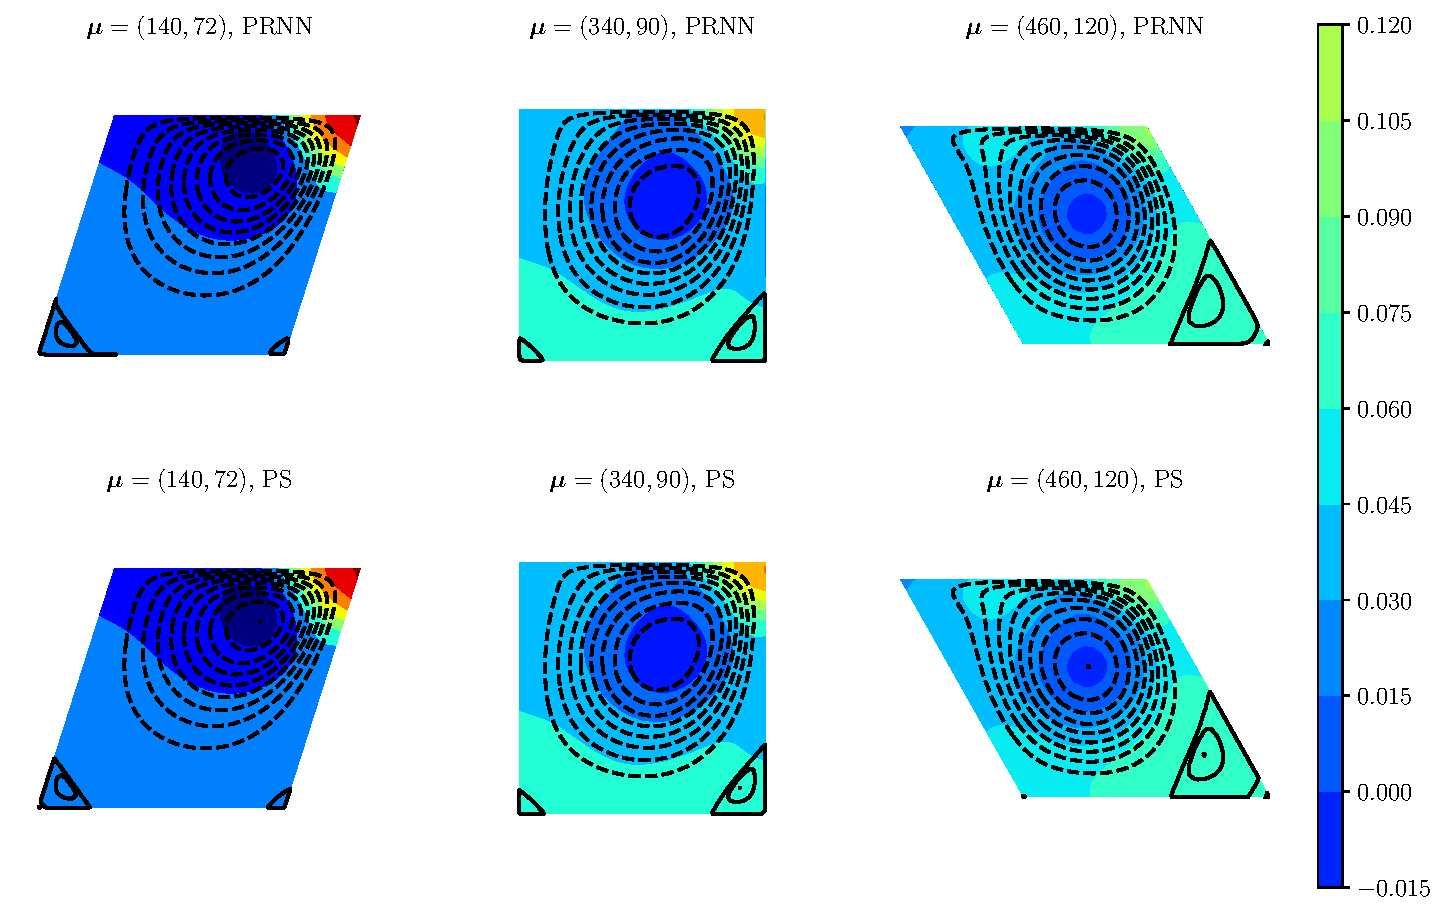
\includegraphics[width=14cm]{../../pythonNN/2DLidDriven/fig/ResultComparsion.pdf}
\caption{The comparison of pressure contour and streamlines of 2D lid-driven flow between the Chebyshev pseudospectral (PS) and the PRNN solutions for four specific parameters. The results of the PRNN are obtained via employing the $m$=25 modes extracted from 100 snapshots and a network of $L$=5 and $n_H$=30 architecture trained with 20000 residual points. The solid streamline indicates an anticlockwise vortex, the dashed streamline an clockwise vortex.}
\label{fig_2DLidDrivenResultComparsion}
\end{figure}





\subsection{Natural convection in enclosure}
To further test the prediction accuracy of the networks for more complex problems, natural convection in enclosure is considered. The geometry and boundary conditions are shown in Fig. \ref{fig_geometry}(b). The unit square cavity is filled with incompressible Newtonian fluid. The cavity is heated and cooled differentially on the two opponent sides, with the other two sides insulated. The gravity acts in the vertical direction. The flow is driven by the vertical buoyancy force, which is modeled according to Boussinesq approximation. The cavity is deployed with a rotation angle $\theta$. To address the variable geometry, a variable coordinate system is applied with $x$-axis perpendicular to the heated/cooled sides.
Thus, the flow is governed by the following two-dimensional incompressible Navier-Stokes equation and energy equation:
\begin{equation}
\left \{
\begin{aligned}
\nabla_{\mathbf{x}}  \cdot {\bf{u}} &= 0 \\
\left( {{\bf{u}} \cdot \nabla_{\mathbf{x}} } \right){\bf{u}} &=  - \nabla_{\mathbf{x}} p + \sqrt{\left(\frac{Pr}{Ra}\right)}{\nabla_{\mathbf{x}} ^2}{\bf{u}} + T\mathbf{n}_g \\
\left( {{\bf{u}} \cdot \nabla_{\mathbf{x}} } \right)T        &=  \frac{1}{\sqrt{\left({Pr}\times{Ra}\right)}}{\nabla_{\mathbf{x}} ^2}T,
\end{aligned}
\right .
,
\label{eq_GoverningEqsNaturalConvection}
\end{equation}
where $\mathbf{u}=(u,v)$ is the dimensionless velocity in Cartesian coordinate $\mathbf{x}=(x,y)$, $p$ is the pressure, $\nabla$ is the  Hamiltonian operator, $Ra$ is the Rayleigh number, $Pr$ is the Prandtl number, $\mathbf{n}_g=\left(\sin(\theta),\cos(\theta) \right)$ is the unit vertical vector. All the sides are no-slip walls. The heated and cooled sides are enforced with the dimensionless temperature $T=0.5$ and $T=-0.5$, respectively. The other two sides are enforced with adiabatic boundary condition $\partial T / \partial y=0$.
Similarly, the flow is solved with the Chebyshev pseudospectral method accompanied with the $IP_{N}-IP_{N-2}$ scheme on a grid of $49 \times 49$.

The parameter space of interest is $\pmb{\mu}=(Ra, Pr, \theta) \in [10^4, 10^5] \times [0.6, 0.8] \times[\pi/4, \pi/2]$. 200 snapshots of high-fidelity solutions for parameters generated with Sobol sequence are calculated and collected for building the reduced basis, and the corresponding singular value distribution is plotted in Fig. \ref{fig_2DNaturalConvectionSingularValues}. It is shown that the singular value decays slowly, implying that more modes are required to represent the underlying dynamic. We choose the first $m=5, 10, 15,...,30$ modes, respectively.
To test the prediction accuracy, a test data set of size $6 \times 6 \times 6=216$ is generated on a tensor-product parameter grid $\pmb{\mu}=\{(1+ 1.8i)\times 10^4\}_{i=0}^{5} \times \{0.6+ 0.04j\}_{j=0}^{5} \times \{\pi/4+ k\pi/20\}_{k=0}^{5}$.
Similarly, for testing the prediction accuracy of the POD-G method, the solving of the reduced-order model for a parameter $\pmb{\mu}$ starts from the projection coefficients of the full-order solution $\pmb{\phi}_h \left( \pmb{\mu} \right)$ on the reduced basis.
For comparison, we pick the first 30, 100 snapshots from the 200 snapshots to do the same test. As for the training of networks, we use the same following hyperparameters: network architecture $L$=5 and $n_H$=30, 40000 epoches, batch size 1000, the leaning rate initialized as 0.01 and decaying by 96\% every 200 epoches.

The prediction accuracy is shown in Fig. \ref{fig_2DNaturalConvectionErrorComparsion_SampleNum}. The tendency of PDNN, PINN and PRNN is similar with that in Fig. \ref{fig_2DLidDrivenErrorComparsion_SampleNum}. Both the PINN and PRNN are much better than the PDNN.  Both the PINN and PRNN can achieve a higher accuracy with 30 snapshots than the PDNN even with 200 snapshots. The PRNN is the best choice, as it not only enjoys a high accuracy, but also shows an improvement with the increase of the snapshots. Besides, the test error of the PRNN is about one order of magnitude smaller than the PDNN for a larger $m$.
The further confirmation of the reliability of PRNN is shown in Fig. \ref{fig_2DNaturalConvectionResultComparsion}, offering a good agreement between the Chebyshev pseudospectral method and the PRNN for some specific parameters. Also, the displayed streamlines are derived from solving Eq. \ref{eq_Streamfunction}.

%\begin{figure}[!ht]
%  \centering
%  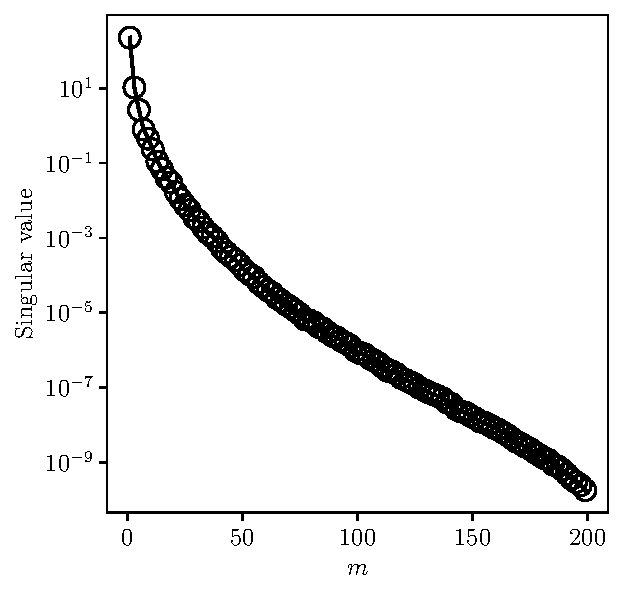
\includegraphics[width=9cm]{../../pythonNN/2DNaturalConvection/fig/SingularValues_200.pdf}
%\caption{Singular value distribution of 200 snapshots for 2D natural convection }
%\label{fig_2DNaturalConvectionSingularValues}
%\end{figure}

\begin{figure}[!ht]
  \centering
  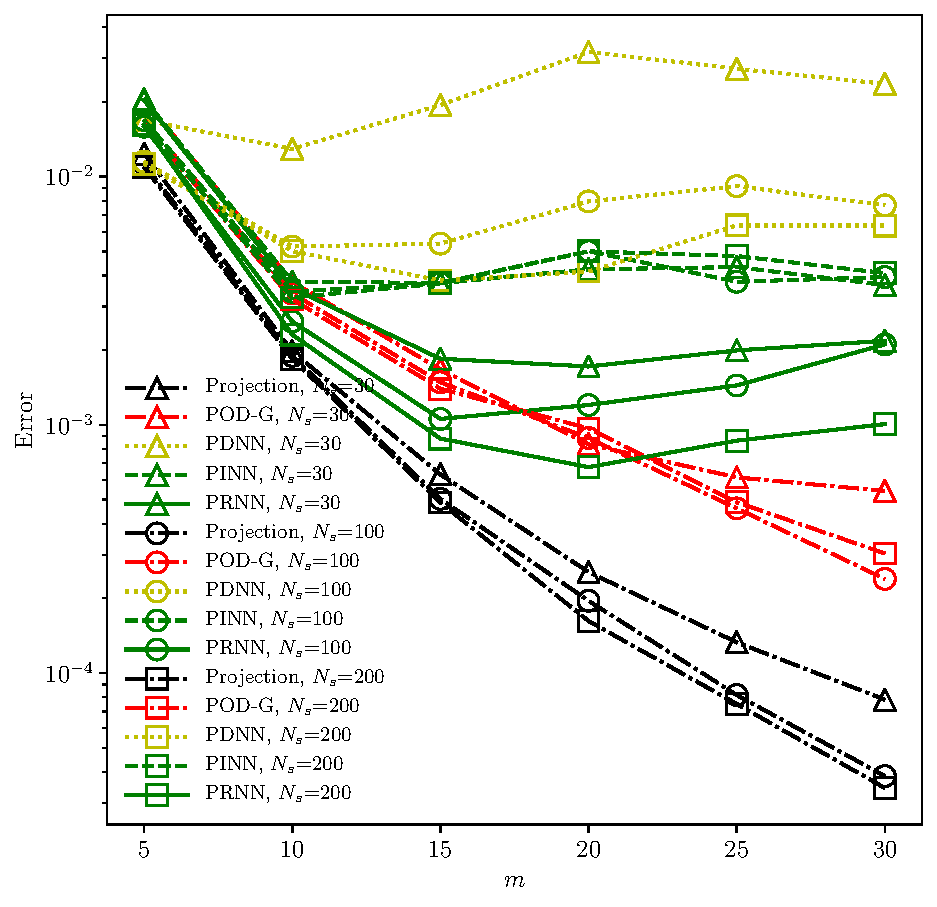
\includegraphics[width=12cm]{../../pythonNN/2DNaturalConvection/fig/ErrorComparsion_SampleNum.pdf}
\caption{The prediction accuracy of the Projection, POD-G, PDNN, PINN and PRNN methods for 2D natural convection with the number of snapshots $N_s$=30, 100 and 200, respectively.}
\label{fig_2DNaturalConvectionErrorComparsion_SampleNum}
\end{figure}

\begin{figure}[!ht]
  \centering
  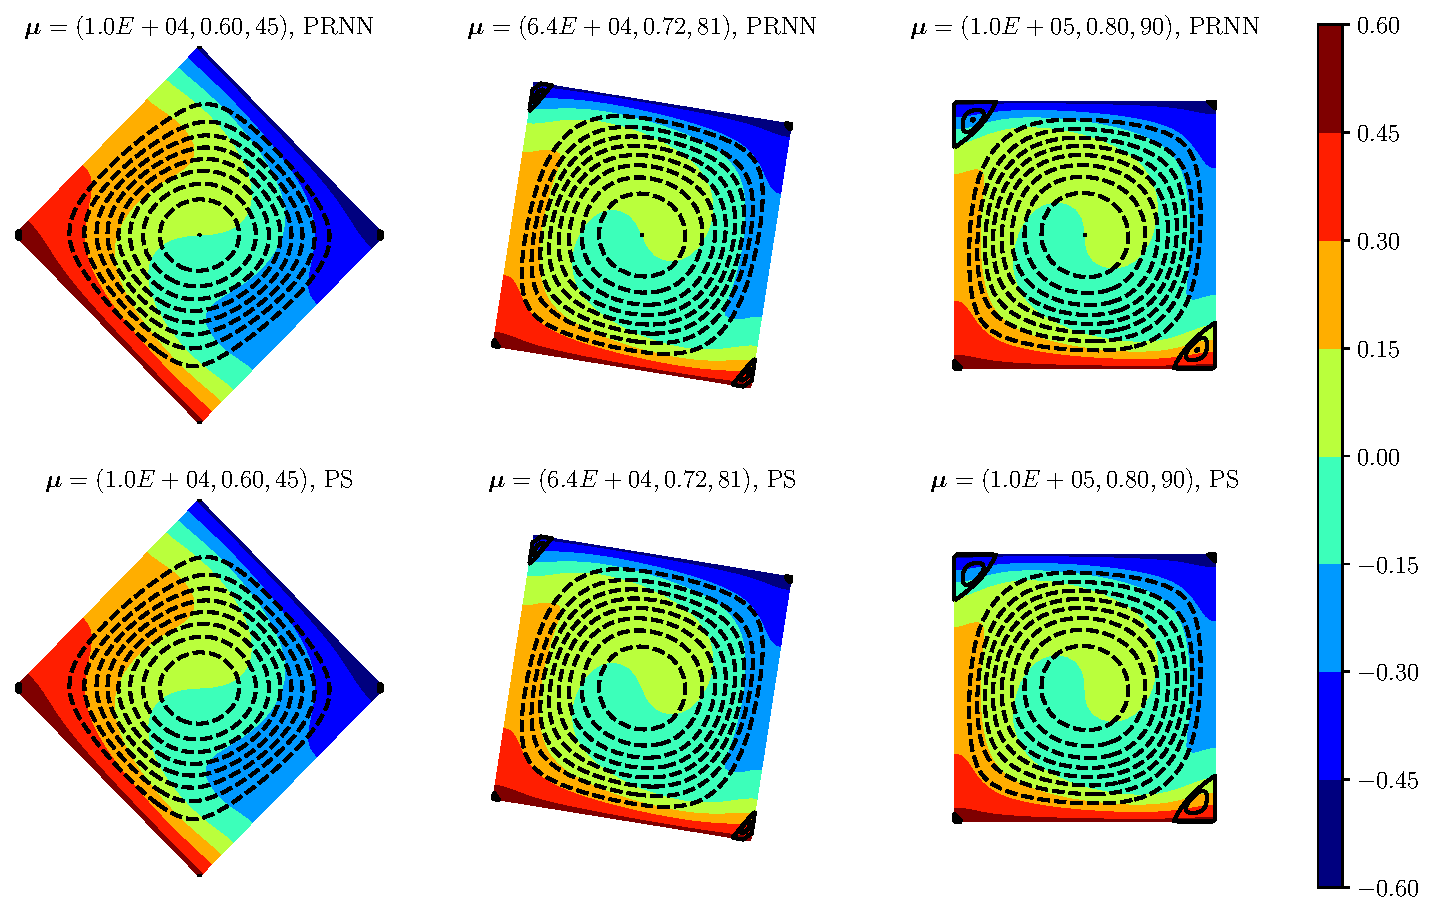
\includegraphics[width=16cm]{../../pythonNN/2DNaturalConvection/fig/ResultComparsion.pdf}
\caption{The comparison of temperature contour and streamlines of 2D natural convection between the Chebyshev pseudospectral (PS) and the PRNN solutions for four specific parameters. The results of the PRNN are obtained via employing the $m$=25 modes extracted from 100 snapshots and a network of $L$=5 and $n_H$=30 architecture trained with 20000 residual points. The solid streamline indicates an anticlockwise vortex, the dashed streamline an clockwise vortex.}
\label{fig_2DNaturalConvectionResultComparsion}
\end{figure}

\FloatBarrier
\section{Conclusions}
This paper proposed a physics-informed machine learning framework for reduced-order modeling of parameterized PDEs.
A reduced space, spanned by the reduced basis extracted by high-fidelity solutions (snapshots), is built for representing the main dynamics of the problem. The full-order model is projected onto the reduced space according to Galerkin method, leading to the reduce-order model.
Combining reduced-order information and marching learning, a physics-informed neural network (PINN) and a physics-reinforced neural network are proposed and trained for approximating the map from parameters to projection coefficients.
The PINN are intended for resolving the reduced-order model directly, while the PRNN are intended for finding somewhere between the reduced-order model and high-fidelity solutions.  The proposed PINN and PRNN  are compared with the Projection method, the POD-G method and  a non-intrusive reduced basis method (referred to PDNN), by testing on three problems: one-dimensional Burges' equation, two-dimensional lid-driven flow and natural convection in enclosure.

The proposed PINN and PRNN both can achieve a higher accuracy with fewer snapshots than the PDNN. For complex nonlinear problems, the PINN sometimes will be trapped with local minima problem, thus limiting its accuracy. On the contrary, the PRNN has no such problems, and its accuracy increases with the number of available snapshots. In particular, once the snapshots are enough for building reduced basis, the PRNN method will promise a satisfactory accuracy.


\section*{Acknowledgments}
The first author is financially supported by Xi'an Jiaotong University Graduate Short-term Academic Visiting Program, National Key Research and Development Project of China [Grant number 2016YFB0200901], National Science and Technology Major Project of China [Grant number 2017-II-0006-0020].

%% References
\section*{References}
\bibliographystyle{elsarticle-num}
\bibliography{ref}

\end{document}
%%\endinput
%%
%% End of file `elsarticle-template-num.tex'.
